% ============================================================
%  The Particle Model — Lesson Booklet (one section per lesson: A Reading · B Theory · C Practice · D Above level)
%  Year 7 (Year 8 extension)  |  Victorian Curriculum F–10 Version 2.0
%  Compile with: xelatex three times, then python3 fill.py Particle_Model_Lesson_Booklet_Yr7
% ============================================================
\documentclass[11pt,a5paper,twoside]{article}

% ── Fonts (compile with LuaLaTeX) ────────────────────────────────────────────
\usepackage{fontspec}
% Bundled fonts (in ./fonts/) so the document compiles anywhere with XeLaTeX/LuaLaTeX
\setmainfont{Lato}[                   % body — humanist sans (stands in for deck's Inter)
  Path=../fonts/, Extension=.ttf, Ligatures=TeX,
  UprightFont=Lato-Regular, ItalicFont=Lato-Italic,
  BoldFont=Lato-Bold, BoldItalicFont=Lato-BoldItalic ]
\newfontfamily\headingfont{Poppins}[  % display/headings — matches the slide decks
  Path=../fonts/, Extension=.ttf, Ligatures=TeX,
  UprightFont=Poppins-Regular, ItalicFont=Poppins-Italic,
  BoldFont=Poppins-Bold, BoldItalicFont=Poppins-BoldItalic ]
\setlength{\headheight}{22pt}

\usepackage[protrusion=true,expansion=false]{microtype}
\usepackage[a5paper, inner=17mm, outer=13mm, top=19mm, bottom=17mm, headheight=14pt, headsep=4mm, footskip=8mm]{geometry}
\usepackage{xcolor}
\usepackage{tikz}
\usetikzlibrary{arrows.meta, shapes.geometric, calc, positioning, decorations.pathreplacing}
\usepackage{tcolorbox}
\tcbuselibrary{skins, breakable, raster}
\usepackage{fancyhdr}
\usepackage{titlesec}
\usepackage{enumitem}
\usepackage{booktabs}
\usepackage{tabularx}
\usepackage{array}
\usepackage{colortbl}
\usepackage{multicol}
\usepackage{amsmath}
\usepackage{needspace}
% TikZ diagram macros are embedded below (just before \begin{document}) for easy editing.
\usepackage{longtable}
\usepackage{graphicx}
\usepackage{lastpage}
\usepackage{calc}
\usepackage{mdframed}
\usepackage{setspace}
\usepackage{ragged2e}
% PDF bookmarks: one per lesson (made in \sectiondiv) plus the cover and
% contents, and links from the contents table to each lesson.
% implicit=false: hyperref adds no anchors of its own (an anchor on each
% list item nudged lists down 1.5 mm, which would undo the page fill).
% hidelinks keeps the links invisible, so the printed pages are unchanged.
\usepackage[implicit=false, hidelinks,
  pdftitle={The Particle Model — Lesson Booklet (A5)},
  pdfsubject={Years 7–8 Science, Victorian Curriculum F–10 v2.0}]{hyperref}
\usepackage{bookmark} % writes the outline itself, which implicit=false switches off in hyperref
% hyperref 7.01 with implicit=false leaves \Hy@PageAnchorSlide undefined, which
% throws at \end{document} and stops fill.py (it builds with -halt-on-error).
\makeatletter\providecommand\Hy@PageAnchorSlide{}\makeatother

% ── Colour Palette ───────────────────────────────────────────────────────────
% Remapped to the slide-deck palette (names kept so body + diagrams cascade)
\definecolor{NavyBlue}   {HTML}{16305C}
\definecolor{MidBlue}    {HTML}{2E6FE0}
\definecolor{LightBlue}  {HTML}{E8F1FF}
\definecolor{TealGreen}  {HTML}{0F6E63}
\definecolor{LightGreen} {HTML}{E0F7F3}
\definecolor{GoldDark}   {HTML}{C77F12}
\definecolor{GoldLight}  {HTML}{FFF3DC}
\definecolor{PurpleDark} {HTML}{5B3FC0}
\definecolor{PurpleLight}{HTML}{EFE9FF}
\definecolor{OrangeDark} {HTML}{C9483D}
\definecolor{OrangeLight}{HTML}{FFE9E6}
\definecolor{MidGrey}    {HTML}{AEBED4}
\definecolor{LightGrey}  {HTML}{F2F5FA}
\definecolor{DarkGrey}   {HTML}{3A4759}
\definecolor{TableHead}  {HTML}{16305C}
\definecolor{RowAlt}     {HTML}{EEF4FF}
% Bright accent tints (deck) for bars, rules and chips
\definecolor{Blue}   {HTML}{2E6FE0}
\definecolor{Teal}   {HTML}{18A999}
\definecolor{Amber}  {HTML}{F5A623}
\definecolor{Coral}  {HTML}{FF6B5E}
\definecolor{Violet} {HTML}{7C5CE0}
\definecolor{Sky}    {HTML}{4DA3FF}
\definecolor{Ink}    {HTML}{16223A}
\definecolor{Line}   {HTML}{DDE5F0}
\definecolor{Paper}  {HTML}{FBFCFE}

% ── Page Style ───────────────────────────────────────────────────────────────
\pagestyle{fancy}
\fancyhf{}
\renewcommand{\headrulewidth}{0.4pt}
\renewcommand{\headrule}{\hbox to\headwidth{\color{NavyBlue}\leaders\hrule height \headrulewidth\hfill}}
\fancyhead[L]{\headingfont\small\color{NavyBlue}The Particle Model}
\fancyhead[R]{\headingfont\small\color{DarkGrey}Year 7 \textbar{} Victorian Curriculum F--10 v2.0}
\fancyfoot[C]{\headingfont\small\color{DarkGrey}\thepage\ \textbar{} \pageref{LastPage}}
\fancypagestyle{plain}{%
  \fancyhf{}
  \fancyfoot[C]{\headingfont\small\color{DarkGrey}\thepage\ \textbar{} \pageref{LastPage}}
  \renewcommand{\headrulewidth}{0pt}
}

% ── Section Formatting ───────────────────────────────────────────────────────
\titleformat{\section}
  {\headingfont\color{NavyBlue}\Large\bfseries}
  {}{0em}{}
  [{\color{Teal}\rule[0.6ex]{2.2em}{3pt}}{\color{Line}\rule[0.6ex]{\dimexpr\linewidth-2.2em\relax}{1pt}}]
\titlespacing{\section}{0pt}{18pt}{8pt}

\titleformat{\subsection}
  {\headingfont\color{MidBlue}\large\bfseries}
  {\thesubsection}{0.6em}{}
\titlespacing{\subsection}{0pt}{12pt}{4pt}

\titleformat{\subsubsection}
  {\headingfont\color{NavyBlue}\normalsize\bfseries}
  {}{0em}{}
\titlespacing{\subsubsection}{0pt}{8pt}{2pt}

% Deck-style eyebrow / kicker (optional use)
\newcommand{\kicker}[2][Teal]{%
  {\headingfont\bfseries\footnotesize\color{#1}%
   \textcolor{#1}{\rule[0.18ex]{1.6em}{2.2pt}}\hspace{0.5em}\MakeUppercase{#2}\par}%
  \vspace{2pt}}

% ── Custom tcolorbox Environments ────────────────────────────────────────────

% Section divider banner
\newtcolorbox{sectionbanner}[2]{
  enhanced, breakable=false,
  colback=NavyBlue, colframe=NavyBlue,
  fontupper=\color{white}\bfseries\large,
  left=4mm, right=4mm, top=3mm, bottom=3mm,
  title={\color{white}\Huge\bfseries #1},
  attach boxed title to top left={yshift=-2mm, xshift=4mm},
  boxed title style={colback=NavyBlue, colframe=NavyBlue},
  after upper={\par\smallskip\normalfont\normalsize\color{white!80!NavyBlue}\textit{#2}}
}

% Key info box (blue)
\newtcolorbox{infobox}[1]{
  breakable, arc=2.5mm, boxrule=0.5pt,
  colback=LightBlue, colframe=Blue!40,
  fonttitle=\headingfont\bfseries, coltitle=MidBlue,
  title={#1},
  left=4mm, right=3.5mm, top=2.5mm, bottom=2.5mm
}

% Scaffold box (yellow)
\newtcolorbox{scaffold}[1]{
  breakable, arc=2.5mm, boxrule=0.5pt,
  colback=GoldLight, colframe=Amber!40,
  fonttitle=\headingfont\bfseries, coltitle=GoldDark,
  title={#1},
  left=4mm, right=3.5mm, top=2.5mm, bottom=2.5mm
}

% Worked example box
\newtcolorbox{workedexbox}[1]{
  breakable, arc=2.5mm, boxrule=0.5pt,
  colback=white, colframe=Amber!50,
  fonttitle=\headingfont\bfseries, coltitle=GoldDark,
  title={#1},
  left=4mm, right=3.5mm, top=2.5mm, bottom=2.5mm
}
% Worked examples: \begin{workedex}{title} -> "Worked Example N.M --- title",
% auto-numbered per section and labelled we:N.M. Never type the number.
\newcounter{wenum}[section]
\renewcommand{\thewenum}{\thesection.\arabic{wenum}}
\newenvironment{workedex}[1]
  {\refstepcounter{wenum}\label{we:\thewenum}\begin{workedexbox}{Worked Example \thewenum\ --- #1}}
  {\end{workedexbox}}

% We do: straight after each worked example, a near-identical question the
% class works through together, with its own writing space. Numbered to
% match the worked example above it and labelled wd:N.M.
%   \begin{wedo}{title} question ... \answerbox{h} \end{wedo}
\newtcolorbox{wedobox}[1]{
  enhanced, breakable=false, arc=2.5mm, boxrule=0.5pt,
  colback=white, colframe=TealGreen!55,
  fonttitle=\headingfont\bfseries, coltitle=TealGreen!75!black,
  title={#1},
  left=4mm, right=3.5mm, top=2.5mm, bottom=2.5mm
}
\newenvironment{wedo}[1]
  {\par\needspace{9\baselineskip}\begin{wedobox}{We do \thewenum\ --- #1}\label{wd:\thewenum}\ignorespaces}
  {\end{wedobox}}

% Year 7 box (blue)
\newtcolorbox{yr7box}{
  breakable, arc=2.5mm, boxrule=0.5pt,
  colback=LightBlue, colframe=Blue!40,
  left=4mm, right=3.5mm, top=2.5mm, bottom=2.5mm
}

% Year 8 extension box (violet)
\newtcolorbox{yr8box}{
  breakable, arc=2.5mm, boxrule=0.5pt,
  colback=PurpleLight, colframe=Violet!40,
  left=4mm, right=3.5mm, top=2.5mm, bottom=2.5mm
}

% Answer lines box
\newcommand{\answerbox}[1]{%
  \begin{tcolorbox}[
    enhanced, breakable, arc=2mm,
    colback=Paper, colframe=Line,
    left=2mm, right=2mm, top=1mm, bottom=1mm,
    boxrule=1pt,
    height=#1
  ]
  \end{tcolorbox}%
}

% Experiment header
\newtcolorbox{expheader}[3]{
  breakable=false, arc=2.5mm,
  colback=RowAlt, colframe=Amber!50, boxrule=0.5pt,
  fonttitle=\headingfont\bfseries\large, coltitle=NavyBlue,
  title={Experiment #1: #2},
  left=4mm, right=3.5mm, top=2.5mm, bottom=2.5mm,
  after upper={\par\smallskip
    {\headingfont\bfseries\color{GoldDark}Aim:}\ \textit{#3}},
}

% Reading comprehension passage box (green)
\newtcolorbox{readingbox}[1]{
  breakable, arc=2.5mm, boxrule=0.5pt,
  colback=white, colframe=Teal!50,
  fonttitle=\headingfont\bfseries, coltitle=TealGreen,
  title={#1},
  left=4mm, right=3.5mm, top=2.5mm, bottom=2.5mm,
  fontupper=\normalsize
}

% Skill-builder box (for beginner scaffolding)
\newtcolorbox{skillbox}[1]{
  breakable, arc=2.5mm, boxrule=0.5pt,
  colback=RowAlt, colframe=Blue!40,
  fonttitle=\headingfont\bfseries, coltitle=MidBlue,
  title={#1},
  left=4mm, right=3.5mm, top=2.5mm, bottom=2.5mm
}

% ── Custom Commands ───────────────────────────────────────────────────────────

% Question: \question{marks}{text}  (marks can be empty)
% Numbered automatically as Q<section>.<n>, reset every section.
% Do NOT write numbers by hand.
\newcounter{qnum}[section]
\renewcommand{\theqnum}{\thesection.\arabic{qnum}}
\newcommand{\question}[2]{%
  \refstepcounter{qnum}%
  \needspace{3\baselineskip}%
  \medskip
  \noindent\label{q:\theqnum}\textbf{Q\theqnum}\ifx&#1&\else\ \textcolor{DarkGrey}{(#1 mark\ifnum#1=1\else s\fi)}\fi\quad #2%
  \medskip
}

% Inline marks note
\newcommand{\markscount}[1]{\hfill\textcolor{DarkGrey}{\textit{(#1 mark\ifnum#1=1\else s\fi)}}}

% ── Practice set counter and question macros ─────────────────────────────────
\newcounter{pqnum}
\newcommand{\practiceset}[1]{%
  \needspace{6\baselineskip}
  \setcounter{pqnum}{0}%
  \vspace{6pt}
  {\headingfont\bfseries\large\color{GoldDark} Practice Set --- #1}\\[-2pt]
  {\color{Amber}\rule{\linewidth}{1pt}}\\[2pt]
}
% \pq{question text}{working box height}
\newcommand{\pq}[2]{%
  \stepcounter{pqnum}%
  \needspace{4\baselineskip}
  \vspace{5pt}
  \noindent\textbf{\thepqnum.}\quad #1\par
  \vspace{2pt}
  \answerbox{#2}
}
% Two short questions side by side, each with its own box
\newcommand{\pqpair}[4]{%
  \needspace{4\baselineskip}
  \vspace{5pt}
  \noindent
  \begin{minipage}[t]{0.48\linewidth}
    \stepcounter{pqnum}\textbf{\thepqnum.}\quad #1\par\vspace{2pt}
    \begin{tcolorbox}[enhanced,arc=2mm,colback=Paper,colframe=Line,left=2mm,right=2mm,
      top=1mm,bottom=1mm,boxrule=1pt,height=#2]\end{tcolorbox}
  \end{minipage}\hfill
  \begin{minipage}[t]{0.48\linewidth}
    \stepcounter{pqnum}\textbf{\thepqnum.}\quad #3\par\vspace{2pt}
    \begin{tcolorbox}[enhanced,arc=2mm,colback=Paper,colframe=Line,left=2mm,right=2mm,
      top=1mm,bottom=1mm,boxrule=1pt,height=#4]\end{tcolorbox}
  \end{minipage}
}

% ── Comprehension question macro (compact, lined) ────────────────────────────
\newcounter{rcnum}
\newcommand{\rcreset}{\setcounter{rcnum}{0}}
\newcommand{\rcq}[2]{%
  \stepcounter{rcnum}%
  \needspace{3\baselineskip}
  \vspace{4pt}
  \noindent\textbf{C\thercnum.}\quad #1\par
  \vspace{2pt}
  \linedbox{#2}
}

% Section divider (big numbered banner): \sectiondiv{title}{summary}
%
% This IS the section: it steps the real section counter, so subsections,
% tasks, questions and figures inside it are numbered N.M automatically.
% Put \label{sec:N} straight after it. Never hand-type a section number.
\newcommand{\sectiondiv}[2]{%
  \needspace{5\baselineskip}%
  \refstepcounter{section}%
  % PDF bookmark for the lesson; its anchor, lesson.N.1, is what the contents table links to
  \pdfbookmark[1]{Lesson \thesection{} — #1}{lesson.\thesection}%
  \begin{tcolorbox}[
    enhanced, breakable=false, arc=3.5mm,
    colback=NavyBlue, colframe=NavyBlue, boxrule=0pt,
    sidebyside, sidebyside align=center,
    lefthand width=2.4cm,
    left=2mm, right=4mm, top=4mm, bottom=4mm
  ]
    \begin{center}
      {\headingfont\bfseries\color{white!35!NavyBlue}\fontsize{50}{50}\selectfont \thesection}
    \end{center}
    \tcblower
    {\headingfont\bfseries\color{white}\LARGE #1}\\[3pt]
    {\itshape\color{white!75!NavyBlue}\small #2}
  \end{tcolorbox}%
}

% Tasks: \task, \task[a] (part a of a NEW task), \taskpart{b} (next part
% of the same task), \exttask (Year 8 "Extension" — same counter).
% Numbered Task <section>.<n>, reset every section. Do NOT type numbers.
% Every task, question and figure also gets an automatic label
% (task:1.7b, q:2.4, fig:1.2, fig:E2.1) so page refs come from the .aux.
\newcounter{tasknum}[section]
\renewcommand{\thetasknum}{\thesection.\arabic{tasknum}}
\NewDocumentCommand{\task}{o}{\refstepcounter{tasknum}\label{task:\thetasknum\IfValueT{#1}{#1}}\textbf{Task \thetasknum\IfValueT{#1}{#1}}}
\newcommand{\taskpart}[1]{\label{task:\thetasknum#1}\textbf{Task \thetasknum#1}}
\newcommand{\exttask}{\refstepcounter{tasknum}\label{task:\thetasknum}\textbf{Extension \thetasknum}}

% Figure captions: \figcap[fig:label]{caption} -> "Figure N.M --- caption"
% \expfigcap{caption} -> "Figure EN.M" (experiment pages). Both auto-numbered.
\newcounter{fignum}[section]
\renewcommand{\thefignum}{\thesection.\arabic{fignum}}
\newcounter{expfignum}[section]
\renewcommand{\theexpfignum}{E\thesection.\arabic{expfignum}}
\newcommand{\figcap}[2][]{%
  \begin{center}
    \refstepcounter{fignum}\label{fig:\thefignum}\if\relax\detokenize{#1}\relax\else\label{#1}\fi
    \small\itshape\color{DarkGrey} Figure \thefignum\ --- #2
  \end{center}%
}
\newcommand{\expfigcap}[1]{%
  \begin{center}
    \refstepcounter{expfignum}\label{fig:\theexpfignum}%
    \small\itshape\color{DarkGrey} Figure \theexpfignum\ --- #1
  \end{center}%
}

% Diagram include
\newcommand{\diagramfig}[3]{%  {filename}{width fraction}{caption}
  \begin{center}
    \includegraphics[width=#2\linewidth]{#1}\\[4pt]
    \small\itshape\color{DarkGrey} #3
  \end{center}%
}

% Table column types
\newcolumntype{L}[1]{>{\RaggedRight\arraybackslash}p{#1}}
\newcolumntype{C}[1]{>{\Centering\arraybackslash}p{#1}}

% Table header colour
\newcommand{\thead}[1]{\cellcolor{TableHead}\color{white}\bfseries #1}
\newcommand{\talt}{\rowcolor{RowAlt}}
\newcommand{\tmid}{\rowcolor{MidGrey}}

% Inline year tags
\newcommand{\tagyr}[1]{%
  \tikz[baseline=-0.5ex]\node[
    rounded corners=2pt,
    fill=#1!20, draw=#1, text=#1,
    inner xsep=4pt, inner ysep=1pt,
    font=\scriptsize\bfseries
  ]{Yr #1 only};}

% Draw answer lines
\newcommand{\anslines}[1]{%
  \vspace{2pt}%
  \foreach \n in {1,...,#1}{%
    \par\noindent\rule{\linewidth}{0.3pt}\vspace{3pt}%
  }%
}

% ── Document ─────────────────────────────────────────────────────────────────
% ── Optional-lesson note, shown under the lesson banner ──────────────────────
\newcommand{\optionalnote}[1]{%
  % the title is a bold lead-in on the first line rather than a title bar,
  % which keeps Lesson 11's reading on the lesson's first page
  \begin{tcolorbox}[enhanced, breakable=false, arc=2.5mm, boxrule=0.5pt,
    colback=PurpleLight, colframe=Violet!50,
    left=4mm, right=3.5mm, top=2mm, bottom=2mm]
  {\headingfont\bfseries\color{PurpleDark}Optional lesson \textbullet{} Year 8 extension.}\enspace #1
  \end{tcolorbox}\vspace{2pt}}


% ══════════════════════════════════════════════════════════════════════════════
%  LESSON STRUCTURE (lesson booklet, Oct 2026)
%  Every lesson runs in the same four parts, in this order:
%    \lessonpart{A}{Reading and comprehension}{Teal}   \label{read:N}
%    \lessonpart{B}{Theory and examples}{Blue}         \label{theory:N}
%    \lessonpart{C}{Practice}{Amber}                    \label{prac:N}
%    \lessonpart{D}{Above level}{Violet}                \label{ext:N}
%  Above-level / higher-order questions live ONLY in Part D, at the end.
% ══════════════════════════════════════════════════════════════════════════════
\newcommand{\lessonpart}[3]{%
  \par\if#1A\needspace{10\baselineskip}\vspace{10pt}\else
    \if#1C\notesfill\fi\clearpage\fi
  \begin{tcolorbox}[enhanced, breakable=false, arc=2mm, boxrule=0pt,
    colback=#3!14, borderline west={4pt}{0pt}{#3},
    left=4mm, right=3mm, top=1.6mm, bottom=1.6mm]
  {\headingfont\bfseries\color{#3!60!black}\large Part #1 \textbullet{} #2}
  \end{tcolorbox}\vspace{2pt}}

% Key vocabulary at the start of each lesson: students copy each definition
% from the vocabulary slide in the lesson's starter. First row = red scaffold.
\newcommand{\vocabhead}{%
  \par\vspace{6pt}%
  \begin{tcolorbox}[enhanced, breakable=false, arc=2mm, boxrule=0pt,
    colback=NavyBlue!10, borderline west={4pt}{0pt}{NavyBlue},
    left=4mm, right=3mm, top=1.6mm, bottom=1.6mm]
  {\headingfont\bfseries\color{NavyBlue}\large Key vocabulary}
  \end{tcolorbox}\vspace{2pt}%
  \noindent Copy the definition of each word from the slide. The first one has been done for you.\par}

% Curriculum codes under a lesson banner
\newcommand{\lessoncodes}[1]{%
  {\small\headingfont\color{DarkGrey}Victorian Curriculum 2.0:\ \textbf{#1}}\par\vspace{4pt}}

% Two short tasks side by side, each with its own working box
% \taskpair{text}{box height}{text}{box height}
% The two boxes line up: the shorter question is padded by the difference in
% text height (measured in a scratch box, task counter restored, no label).
\newsavebox\tpbox
\newlength\tpA \newlength\tpB
\newcount\tpsaved
\newcommand\tpmeasure[2]{%
  \tpsaved=\value{tasknum}%
  \sbox\tpbox{\vbox{\hsize=0.485\linewidth \linewidth=\hsize \parskip=0pt
    \renewcommand\label[1]{}\task #1\par}}%
  \setlength{#2}{\dimexpr\ht\tpbox+\dp\tpbox\relax}%
  \setcounter{tasknum}{\tpsaved}}
\newcommand{\taskpair}[4]{%
  \par\needspace{9\baselineskip}\vspace{4pt}%
  \tpmeasure{#1}{\tpA}\tpmeasure{#3}{\tpB}%
  \noindent
  \edef\abgrp{\number\numexpr\value{abox}+1\relax}%
  \begin{minipage}[t]{0.485\linewidth}
    \task #1\par\ifdim\tpB>\tpA\vspace{\dimexpr\tpB-\tpA\relax}\fi\vspace{2pt}\answerbox{#2}
  \end{minipage}\hfill
  \begin{minipage}[t]{0.485\linewidth}
    \task #3\par\ifdim\tpA>\tpB\vspace{\dimexpr\tpA-\tpB\relax}\fi\vspace{2pt}\answerbox{#4}
  \end{minipage}\par\gdef\abgrp{0}\vspace{4pt}}
% Two parts of one question side by side, with their answer boxes level:
% \ptpair{a}{part (a) text}{box height}{b}{part (b) text}{box height}.
% The shorter part's text gets space below it to match the longer one.
\newcommand\ptmeasure[3]{%
  \sbox\tpbox{\vbox{\hsize=0.485\linewidth \linewidth=\hsize \parskip=0pt \pt{#1}#2\par}}%
  \setlength{#3}{\dimexpr\ht\tpbox+\dp\tpbox\relax}}
\newcommand{\ptpair}[6]{%
  \ptmeasure{#1}{#2}{\tpA}\ptmeasure{#4}{#5}{\tpB}%
  \par\noindent
  \edef\abgrp{\number\numexpr\value{abox}+1\relax}%
  \begin{minipage}[t]{0.485\linewidth}
    \pt{#1}#2\par\ifdim\tpB>\tpA\vspace{\dimexpr\tpB-\tpA\relax}\fi\answerbox{#3}
  \end{minipage}\hfill
  \begin{minipage}[t]{0.485\linewidth}
    \pt{#4}#5\par\ifdim\tpA>\tpB\vspace{\dimexpr\tpA-\tpB\relax}\fi\answerbox{#6}
  \end{minipage}\par\gdef\abgrp{0}}

% Answer boxes never split across a page (a half box on its own page is useless)
% ── Page filling ────────────────────────────────────────────────────────────
% Every writing box gets an id. Its page is logged to \jobname.abp; fill.py
% measures the empty space left at the foot of each page and shares it out
% among that page's boxes via \jobname.abx (\abset{id}{extra}). Side-by-side
% boxes share a group so they grow together.
\newcounter{abox}
\newwrite\abpos \immediate\openout\abpos=\jobname.abp
\newcommand{\abset}[2]{\expandafter\gdef\csname abx@#1\endcsname{#2}}
\InputIfFileExists{\jobname.abx}{}{}
\def\abgrp{0}
\newcommand{\abnext}{\stepcounter{abox}%
  \edef\abcur{\ifcsname abx@\theabox\endcsname\csname abx@\theabox\endcsname\else 0pt\fi}}
\newcommand{\ablog}{\edef\abtmp{\noexpand\write\abpos{\theabox\space\abgrp\space\noexpand\thepage}}\abtmp}
\newcommand{\abh}[1]{\dimexpr#1+\abcur\relax}
\renewcommand{\answerbox}[1]{%
  \abnext
  \begin{tcolorbox}[enhanced, breakable=false, arc=2mm, colback=Paper, colframe=Line,
    left=2mm, right=2mm, top=1mm, bottom=1mm, boxrule=1pt, height=\abh{#1}]
  \end{tcolorbox}\ablog%
}
% \linedbox{height}: an answer box ruled in dotted thirds. Lines are \thirdrow/3 apart and run dotted, dotted,
% solid (the baseline), repeating, and end on one dotted line. The number of
% rows is worked out from the box's final height, so the ruling still fills the
% box after fill.py has grown it; the rows are centred in the box.
\newlength\thirdrow \setlength\thirdrow{9mm}
\tikzset{thirdsolid/.style={draw=DarkGrey!70, line width=0.5pt},
         thirddot/.style={draw=DarkGrey!70, line width=0.6pt, dash pattern=on 0.9pt off 1.6pt}}
\newlength\lbH \newlength\lbO \newcount\lbN
\newcommand{\linedbox}[1]{%
  \abnext
  % interior height = box height less the 1pt frame top and bottom
  \setlength\lbH{\dimexpr\abh{#1}-2pt\relax}%
  % whole rows that fit with at least 3 mm spare top and bottom (at least one)
  \lbN=\numexpr(\dimexpr\lbH-6mm-\thirdrow/2\relax)/\thirdrow\relax
  \ifnum\lbN<1 \lbN=1 \fi
  \setlength\lbO{\dimexpr(\lbH-\lbN\thirdrow)/2\relax}%
  \begin{tcolorbox}[enhanced, breakable=false, arc=2mm, colback=Paper, colframe=Line,
    left=2mm, right=2mm, top=1mm, bottom=1mm, boxrule=1pt, height=\abh{#1},
    underlay={\begin{tcbclipinterior}
      \foreach \i in {1,...,\the\lbN}{
        \draw[thirddot] ([xshift=3mm,yshift=-\lbO-(\i-1)*\thirdrow]interior.north west) -- ([xshift=-3mm,yshift=-\lbO-(\i-1)*\thirdrow]interior.north east);
        \draw[thirddot] ([xshift=3mm,yshift=-\lbO-(\i-1)*\thirdrow-\thirdrow/3]interior.north west) -- ([xshift=-3mm,yshift=-\lbO-(\i-1)*\thirdrow-\thirdrow/3]interior.north east);
        \draw[thirdsolid] ([xshift=3mm,yshift=-\lbO-(\i-1)*\thirdrow-2*\thirdrow/3]interior.north west) -- ([xshift=-3mm,yshift=-\lbO-(\i-1)*\thirdrow-2*\thirdrow/3]interior.north east);}
      \draw[thirddot] ([xshift=3mm,yshift=-\lbO-\lbN\thirdrow]interior.north west) -- ([xshift=-3mm,yshift=-\lbO-\lbN\thirdrow]interior.north east);
    \end{tcbclipinterior}}]
  \end{tcolorbox}\ablog%
}
% Every written-response box is ruled the same way (Part A comprehension, We do,
% Part C tasks and Part D extensions, including side-by-side pairs). Space for
% mathematical working uses \workbox{height} instead and stays plain, as do
% \drawbox and the write-in tables.
\let\workbox\answerbox   % plain box: mathematical working (calculations) stays unruled
\let\answerbox\linedbox
% \drawbox{height}{contents}: white box for a diagram or drawing
\newcommand{\drawbox}[2]{%
  \abnext
  \begin{tcolorbox}[colback=white, colframe=MidGrey, boxrule=0.5pt, height=\abh{#1}]#2\end{tcolorbox}\ablog}
% Notes box at the end of Part B: fills whatever is left of the page (if worth it)
\newcommand{\notesfill}{\par
  \ifdim\dimexpr\pagegoal-\pagetotal\relax>3.2cm
    \vspace*{\fill}%
    \begin{tcolorbox}[enhanced, breakable=false, arc=2mm, colback=Paper, colframe=Line,
      left=2mm, right=2mm, top=1mm, bottom=1mm, boxrule=1pt,
      height=\dimexpr\pagegoal-\pagetotal-1.0cm\relax]
      {\small\headingfont\color{DarkGrey}Notes}
    \end{tcolorbox}%
  \fi}



% Centred table: wrap every content table in \begin{ctab} ... \end{ctab}
% (figures already centre themselves inside their \diag... macros)
% ctab also registers write-in tables (S column) for page filling: the extra
% height is per row, logged with the row count.
\newenvironment{ctab}{\par\smallskip\begingroup\centering
  \abnext\let\tbcur\abcur\global\wtrows0 }{\par
  \ifnum\wtrows>0 \edef\abtmp{\noexpand\write\abpos{\theabox\space\abgrp\space\noexpand\thepage\space\the\wtrows}}\abtmp\fi
  \endgroup\smallskip}

% ── Booklet formatting rules (Oct 2026) ─────────────────────────────────────
% 1. No marks are shown anywhere in the booklet.
\renewcommand{\markscount}[1]{}
% 2. A task's heading sits on its own line; its text starts on the next
%    line, left aligned. Parts (a), (b)… each start a new line: use \pt{a}.
\RenewDocumentCommand{\task}{o}{\par\noindent\refstepcounter{tasknum}\label{task:\thetasknum\IfValueT{#1}{#1}}\textbf{Task \thetasknum\IfValueT{#1}{#1}}\par\nobreak\noindent\ignorespaces}
\renewcommand{\taskpart}[1]{\par\noindent\label{task:\thetasknum#1}\textbf{Task \thetasknum#1}\par\nobreak\noindent\ignorespaces}
\renewcommand{\exttask}{\par\noindent\refstepcounter{tasknum}\label{task:\thetasknum}\textbf{Extension \thetasknum}\par\nobreak\noindent\ignorespaces}
\newcommand{\pt}[1]{\par\noindent\textbf{(#1)}\ \ignorespaces}
% Workstation pages (Experiment 1): numbered method steps with a hanging
% indent, and a one-line safety reminder under the materials list.
\newcommand{\wsstep}[1]{\par\noindent\hangindent=1.6em\hangafter=1\makebox[1.6em][l]{\textbf{#1}}\ignorespaces}
\newcommand{\wssafety}[1]{\par\smallskip{\small\textcolor{ScaffoldRed}{\headingfont\bfseries Safety:}\ #1}\par}
% 3. Tables have vertical rules between columns and down both sides
%    (write | between and around the columns, e.g. {|L{3cm}|C{2cm}|}).
%    Keep the normal padding at the outer edges (no @{} there): colortbl paints
%    header colour one \tabcolsep past each edge, so trimming the padding makes
%    the header overhang the grid.
\arrayrulecolor{MidGrey}
\setlength{\arrayrulewidth}{0.6pt}
% 4. Write-in tables: W/Z are left/centred columns that centre text
%    vertically; put the S column first (see below).
\newcolumntype{W}[1]{>{\RaggedRight\arraybackslash}m{#1}}
\newcolumntype{Z}[1]{>{\Centering\arraybackslash}m{#1}}
\def\tbcur{0pt}
\newcount\wtrows
\newcommand{\wh}{\global\advance\wtrows1 \rule[\dimexpr-0.75cm-\tbcur/2\relax]{0pt}{\dimexpr1.5cm+\tbcur\relax}}
% S = zero-width first column that makes every row of a write-in table
% at least 1.5 cm tall with its text vertically centred. Start each data
% row with "&"; start the header row with "\hd &" so it stays slim.
\newif\ifnowh
\newcolumntype{S}{@{}>{}c<{\ifnowh\else\wh\fi\global\nowhfalse}@{\hspace{\tabcolsep}}}
\newcommand{\hd}{\global\nowhtrue}
% 5. The first row of a multi-row write-in table is a worked scaffold in red.
\definecolor{ScaffoldRed}{HTML}{C0392B}
\newcommand{\scaf}[1]{\textcolor{ScaffoldRed}{\itshape #1}}
% 6. Tables are a light grid (rules between rows and columns) on white —
%    row shading is off, because colortbl paints shading over column rules.
\renewcommand{\talt}{}
\renewcommand{\tmid}{}
% ══════════════════════════════════════════════════════════════════════════════
%  DIAGRAM DEFINITIONS — The Particle Model
%  Self-contained TikZ macros, no external image files. Each \diag... macro is
%  called from the body by name.
% ══════════════════════════════════════════════════════════════════════════════
\usetikzlibrary{arrows.meta,calc,positioning,patterns,backgrounds}
\tikzset{
  thin arrow/.style={-{Stealth[length=6pt,width=4pt]}, line width=1.4pt},
}

% ── Lesson 1: the same three jars holding a solid, a liquid and a gas ───────────
% The solid keeps its own shape, the liquid takes the jar's shape with a flat top,
% the gas fills the whole jar. No particles yet: those arrive in Lesson 4.
\newcommand{\jar}[1]{% jar outline with its base at (#1,0)
  \draw[line width=1.2pt, Ink] (#1-1.25,2.9) -- (#1-1.25,0.15) arc (180:270:0.15)
    -- (#1+1.1,0) arc (270:360:0.15) -- (#1+1.25,2.9);}
\newcommand{\diagStates}{%
\begin{center}
\begin{fitbox}\begin{tikzpicture}[font=\small, x=1cm, y=1cm]
  % solid: a block sitting in the corner
  \fill[GoldLight] (-0.95,0.02) rectangle (0.15,1.25);
  \draw[GoldDark, line width=1.1pt] (-0.95,0.02) rectangle (0.15,1.25);
  \jar{0}
  \node[font=\bfseries, text=NavyBlue] at (0,-0.45) {Solid};
  \node[align=center, font=\footnotesize, text=DarkGrey] at (0,-1.05) {keeps its own shape\\and volume};
  % liquid: takes the jar's shape, flat top
  \begin{scope}[xshift=4.2cm]
    \fill[Sky!35] (-1.25,0.15) arc (180:270:0.15) -- (1.1,0) arc (270:360:0.15) -- (1.25,1.1) -- (-1.25,1.1) -- cycle;
    \draw[MidBlue, line width=1.1pt] (-1.25,1.1) -- (1.25,1.1);
    \jar{0}
    \node[font=\bfseries, text=NavyBlue] at (0,-0.45) {Liquid};
    \node[align=center, font=\footnotesize, text=DarkGrey] at (0,-1.05) {takes the jar's shape,\\keeps its volume};
  \end{scope}
  % gas: fills the whole (sealed) jar
  \begin{scope}[xshift=8.4cm]
    \fill[Violet!16] (-1.25,0.15) arc (180:270:0.15) -- (1.1,0) arc (270:360:0.15) -- (1.25,2.9) -- (-1.25,2.9) -- cycle;
    \draw[line width=2.2pt, DarkGrey] (-1.4,2.9) -- (1.4,2.9);
    \jar{0}
    \node[font=\scriptsize, text=DarkGrey, anchor=south] at (0,2.95) {lid};
    \node[font=\bfseries, text=NavyBlue] at (0,-0.45) {Gas};
    \node[align=center, font=\footnotesize, text=DarkGrey] at (0,-1.05) {spreads out to fill\\the whole jar};
  \end{scope}
\end{tikzpicture}\end{fitbox}
\end{center}}

% ── Lesson 1, Worked Example 1.2 and We do 1.2: the same syringe, before and after
\newcommand{\diagSyringe}[3]{% {start mL}{end mL}{contents: gas|liquid}
\begin{center}\resizebox{\linewidth}{!}{%
\begin{fitbox}\begin{tikzpicture}[font=\scriptsize, x=0.11cm, y=1cm]
  \foreach \row/\vol/\lab in {0/#1/before, -1.15/#2/after}{
    \begin{scope}[yshift=\row cm]
      \ifx#3g\fill[Violet!16] (0,0) rectangle (\vol,0.7);\else\fill[Sky!35] (0,0) rectangle (\vol,0.7);\fi
      \draw[line width=1pt, Ink] (0,0) rectangle (60,0.7);
      \draw[line width=1pt, Ink] (0,0.25) -- (-4,0.25) (0,0.45) -- (-4,0.45);
      \fill[Ink] (-5.5,0.15) rectangle (-4,0.55);
      \foreach \t in {0,10,...,60}{\draw[Ink] (\t,0.7) -- (\t,0.85); \node[anchor=south, font=\tiny] at (\t,0.82) {\t};}
      \fill[DarkGrey] (\vol,0.04) rectangle (\vol+1.6,0.66);
      \draw[line width=2pt, DarkGrey] (\vol+1.6,0.35) -- (\vol+26,0.35);
      \draw[line width=2pt, DarkGrey] (\vol+26,0.05) -- (\vol+26,0.65);
      \node[anchor=east, font=\scriptsize\bfseries, text=DarkGrey] at (-7,0.35) {\lab};
    \end{scope}}
  \node[font=\tiny, text=DarkGrey, anchor=west] at (61,0.35) {mL};
  \node[font=\tiny, text=DarkGrey, anchor=north] at (-4.75,-1.2) {sealed tip};
\end{tikzpicture}\end{fitbox}}
\end{center}}

% needspace.sty reserves room by planting a penalty -100 with 9 lines of
% temporary stretch. On a page that can't be filled tightly that fake break
% always wins, so a We do that fitted was pushed over and left half a page
% empty. This version breaks only when the room really isn't there, and
% ragged bottom lets every other page run on until something won't fit;
% fill.py then grows the writing boxes into what is left at the foot.
\renewcommand{\needspace}[1]{\par\ifdim\dimexpr\pagegoal-\pagetotal\relax<\dimexpr#1\relax\newpage\fi}
\raggedbottom
% Part D sits in a breakable yr8box, where \needspace can't see the page (the box
% is built off the page first). Wrap each extension in keepext so it is one
% unsplittable block: the yr8box then breaks between extensions, never inside one.
\newenvironment{keepext}{\par\begin{tcolorbox}[blankest, breakable=false]}{\end{tcolorbox}\par}
% ══════════════════════════════════════════════════════════════════════════════
%  SHARED DIAGRAMS — particle boxes, graphs and lab apparatus (Lessons 2–27)
% ══════════════════════════════════════════════════════════════════════════════
% Particles are 3.2 mm discs. Solids and liquids hold about the same number of
% particles at the same spacing (touching): a liquid is NOT drawn more spread
% out than a solid, because that is the misconception Lesson 6 corrects.
\tikzset{
  pA/.style={circle, fill=Sky!55, draw=MidBlue, line width=0.5pt, minimum size=3.2mm, inner sep=0pt},
  pB/.style={circle, fill=Coral!50, draw=OrangeDark, line width=0.5pt, minimum size=3.2mm, inner sep=0pt},
  pC/.style={circle, fill=Amber!55, draw=GoldDark, line width=0.5pt, minimum size=3.2mm, inner sep=0pt},
  pD/.style={circle, fill=Teal!45, draw=TealGreen, line width=0.5pt, minimum size=3.2mm, inner sep=0pt},
  move/.style={-{Stealth[length=3pt,width=3pt]}, line width=0.7pt, DarkGrey},
  boxline/.style={line width=1pt, Ink},
  axis/.style={-{Stealth[length=5pt,width=4pt]}, line width=0.9pt, Ink},
  glass/.style={line width=1pt, Ink},
  lab/.style={font=\scriptsize, text=DarkGrey},
}
\makeatletter
% particle kinds, drawn at (#1,#2): A, B, C, D single particles; AA, BB, CC
% two joined; AB a joined pair; BAB a three-particle molecule.
\newcommand{\pk@A}[2]{\node[pA] at (#1,#2) {};}
\newcommand{\pk@B}[2]{\node[pB] at (#1,#2) {};}
\newcommand{\pk@C}[2]{\node[pC] at (#1,#2) {};}
\newcommand{\pk@D}[2]{\node[pD] at (#1,#2) {};}
\newcommand{\pk@AA}[2]{\node[pA] at ($(#1,#2)+(-0.13,0)$) {};\node[pA] at ($(#1,#2)+(0.13,0)$) {};}
\newcommand{\pk@BB}[2]{\node[pB] at ($(#1,#2)+(-0.13,0)$) {};\node[pB] at ($(#1,#2)+(0.13,0)$) {};}
\newcommand{\pk@CC}[2]{\node[pC] at ($(#1,#2)+(-0.13,0)$) {};\node[pC] at ($(#1,#2)+(0.13,0)$) {};}
\newcommand{\pk@AB}[2]{\node[pA] at ($(#1,#2)+(-0.13,0)$) {};\node[pB] at ($(#1,#2)+(0.13,0)$) {};}
\newcommand{\pk@BAB}[2]{\node[pB] at ($(#1,#2)+(-0.24,0)$) {};\node[pB] at ($(#1,#2)+(0.24,0)$) {};\node[pA] at (#1,#2) {};}
\newcommand{\pk}[3]{\csname pk@#1\endcsname{#2}{#3}}
\makeatother
% eight spread-out positions in a 2.6 cm box (for gases and particle diagrams)
\def\gaspos{0.55/0.55,1.55/0.45,2.15/1.05,0.75/1.35,1.65/1.5,0.5/2.1,2.1/2.15,1.3/2.05}
% the box: a 2.6 cm square with its bottom-left corner at the scope origin
\newcommand{\pbox}{\draw[boxline] (0,0) rectangle (2.6,2.6);}
% \pkinds{A,A,AB,...}: up to eight particles, placed at the eight gas positions
\newcommand{\pkinds}[1]{%
  \foreach \k [count=\i] in {#1}{%
    \foreach \x/\y [count=\j] in \gaspos{\ifnum\i=\j \pk{\k}{\x}{\y}\fi}}}
% \stateIn{solid|liquid|gas}{style} — the particles of one state, in a box
\newcommand{\stateIn}[2]{%
  \ifstrequal{#1}{solid}{%
    \foreach \r in {0,...,4}{\foreach \c in {0,...,6}{\node[#2] at (0.31+\c*0.33,0.2+\r*0.33) {};}}}{}%
  \ifstrequal{#1}{liquid}{%
    \foreach \x/\y in {2.29/0.20,0.42/0.20,1.28/0.20,0.85/0.20,1.87/0.20,1.07/0.47,1.45/0.49,0.28/0.51,0.72/0.52,2.34/0.54,1.87/0.54,1.29/0.80,2.03/0.85,0.27/0.86,0.69/0.86,1.68/0.90,2.34/0.98,0.88/1.15,2.01/1.20,1.63/1.24,0.55/1.26,1.18/1.31,2.36/1.33,0.23/1.39,0.88/1.50,1.99/1.55,1.65/1.59,0.51/1.61,1.30/1.63}{\node[#2] at (\x,\y) {};}}{}%
  \ifstrequal{#1}{gas}{%
    \foreach \x/\y in \gaspos{\node[#2] at (\x,\y) {};}}{}%
  \pbox}
% motion marks: short arrows for a gas, small wiggles for a solid
\newcommand{\gasMoves}{%
  \draw[move] (0.55,0.55)+(0.2,0.12) -- +(0.55,0.33);
  \draw[move] (1.55,0.45)+(-0.2,0.08) -- +(-0.55,0.25);
  \draw[move] (2.15,1.05)+(0,0.2) -- +(0.05,0.55);
  \draw[move] (0.75,1.35)+(0.2,-0.08) -- +(0.55,-0.2);
  \draw[move] (1.65,1.5)+(-0.18,0.12) -- +(-0.45,0.4);
  \draw[move] (0.5,2.1)+(0.08,-0.2) -- +(0.2,-0.52);
  \draw[move] (2.1,2.15)+(-0.2,-0.05) -- +(-0.55,-0.15);
  \draw[move] (1.3,2.05)+(0.12,0.15) -- +(0.3,0.38);}
\newcommand{\solidWiggles}{%
  \foreach \c in {1,3,5}{\draw[DarkGrey, line width=0.5pt] (0.31+\c*0.33-0.14,1.86) -- ++(0.07,0.06) -- ++(0.07,-0.06) -- ++(0.07,0.06) -- ++(0.07,-0.06);}}
\newcommand{\liquidMoves}{%
  \draw[move] (0.88,1.5)+(0.18,0.05) -- +(0.42,0.12);
  \draw[move] (1.99,1.55)+(-0.18,0.06) -- +(-0.42,0.14);
  \draw[move] (0.55,1.26)+(-0.05,0.18) -- +(-0.1,0.4);}

% Figure: the three states side by side, with movement marks
\newcommand{\diagThreeStates}{%
\begin{center}\begin{fitbox}\begin{tikzpicture}[font=\small]
  \begin{scope}\stateIn{solid}{pA}\solidWiggles\end{scope}
  \begin{scope}[xshift=4.2cm]\stateIn{liquid}{pA}\liquidMoves\end{scope}
  \begin{scope}[xshift=8.4cm]\stateIn{gas}{pA}\gasMoves\end{scope}
  \foreach \x/\t/\d in {1.3/Solid/{packed in a pattern,\\vibrate in place}, 5.5/Liquid/{close together, slide\\past each other}, 9.7/Gas/{far apart, move fast\\in every direction}}{
    \node[font=\bfseries, text=NavyBlue] at (\x,-0.35) {\t};
    \node[align=center, font=\footnotesize, text=DarkGrey] at (\x,-0.95) {\d};}
\end{tikzpicture}\end{fitbox}\end{center}}

% \pboxfig{tikz contents}{label}: one small labelled box (for tasks)
\newcommand{\pboxfig}[2]{%
  \begin{fitbox}\begin{tikzpicture}[baseline=(b.base)]#1\pbox
    \node[font=\small\bfseries, text=NavyBlue] (b) at (1.3,-0.35) {#2};\end{tikzpicture}\end{fitbox}}

% graph-paper box for drawing a graph: \graphgrid{height}
\newcommand{\graphgrid}[1]{%
  \begin{tcolorbox}[enhanced, breakable=false, colback=white, colframe=MidGrey, boxrule=0.5pt, height=#1,
    underlay={\begin{tcbclipinterior}\draw[step=5mm, Line, very thin] (interior.south west) grid (interior.north east);
      \draw[step=1cm, MidGrey!70, thin] (interior.south west) grid (interior.north east);\end{tcbclipinterior}}]
  \end{tcolorbox}}

% Heating curve for water, -20 °C ice to steam at 120 °C. #1 = labels on (1) / off (0)
\newcommand{\diagHeatingCurve}[1]{%
\begin{center}\begin{fitbox}\begin{tikzpicture}[x=0.95cm, y=0.032cm, font=\footnotesize]
  \foreach \t in {-20,0,20,...,120}{\draw[Line] (0,\t) -- (11,\t); \node[anchor=east, text=DarkGrey] at (0,\t) {\t};}
  \foreach \m in {0,...,11}{\draw[Line] (\m,-20) -- (\m,120);}
  \foreach \m in {0,2,...,10}{\node[anchor=north, text=DarkGrey] at (\m,-20) {\m};}
  \draw[axis] (0,-20) -- (11.4,-20) node[anchor=north east, yshift=-12pt, text=Ink] {time (minutes)};
  \draw[axis] (0,-20) -- (0,132) node[anchor=south, text=Ink] {temperature (\textdegree C)};
  \draw[line width=1.8pt, OrangeDark, line join=round] (0,-20) -- (1,0) -- (3,0) -- (6,100) -- (10,100) -- (11,120);
  \ifnum#1=1
    \node[anchor=south, align=center, font=\scriptsize\bfseries, text=MidBlue] at (2,4) {melting};
    \node[anchor=south, align=center, font=\scriptsize\bfseries, text=MidBlue] at (8,104) {boiling};
    \node[anchor=west, font=\scriptsize, text=DarkGrey] at (0.55,-14) {ice warms};
    \node[anchor=west, font=\scriptsize, text=DarkGrey] at (4.3,45) {water warms};
    \node[anchor=east, font=\scriptsize, text=DarkGrey] at (10.9,123) {steam};
  \fi
\end{tikzpicture}\end{fitbox}\end{center}}

% Solubility curves (grams that dissolve in 100 g of water). #1 = which curves:
% 1 = potassium nitrate and salt, 2 = potassium nitrate only
\newcommand{\diagSolubility}[1]{%
\begin{center}\begin{fitbox}\begin{tikzpicture}[x=0.11cm, y=0.024cm, font=\footnotesize]
  \foreach \s in {0,20,...,240}{\draw[Line] (0,\s) -- (100,\s); \node[anchor=east, text=DarkGrey] at (0,\s) {\s};}
  \foreach \s in {10,30,...,230}{\draw[Line!60] (0,\s) -- (100,\s);}
  \foreach \t in {0,10,...,100}{\draw[Line] (\t,0) -- (\t,250); \node[anchor=north, text=DarkGrey] at (\t,0) {\t};}
  \draw[axis] (0,0) -- (104,0) node[anchor=north east, yshift=-12pt, text=Ink] {temperature (\textdegree C)};
  \draw[axis] (0,0) -- (0,262) node[anchor=south west, xshift=-14pt, text=Ink] {solubility (g per 100 g of water)};
  \draw[line width=1.6pt, OrangeDark] plot[smooth] coordinates {(0,13.3) (10,20.9) (20,31.6) (30,45.8) (40,63.9) (50,85.5) (60,110) (70,138) (80,169) (90,202) (100,246)};
  \node[anchor=west, font=\scriptsize\bfseries, text=OrangeDark] at (28,150) {potassium nitrate};
  \ifnum#1=1
    \draw[line width=1.6pt, MidBlue] plot[smooth] coordinates {(0,35.7) (20,36.0) (40,36.6) (60,37.3) (80,38.4) (100,39.8)};
    \node[anchor=south, font=\scriptsize\bfseries, text=MidBlue] at (86,40) {salt};
  \fi
\end{tikzpicture}\end{fitbox}\end{center}}

% Measuring cylinder: \cylinder{x}{liquid level mL}{with rock 0/1}; 0–100 mL scale
\newcommand{\cylinder}[3]{%
  \begin{scope}[xshift=#1cm]
    \fill[Sky!30] (0,0) rectangle (1.2,{#2*0.045});
    \draw[MidBlue, line width=0.8pt] (0,{#2*0.045}) -- (1.2,{#2*0.045});
    \ifnum#3=1 \draw[fill=DarkGrey!45, draw=DarkGrey] (0.3,0.04) -- (0.85,0.06) -- (0.95,0.42) -- (0.6,0.6) -- (0.25,0.38) -- cycle;\fi
    \draw[glass] (0,4.8) -- (0,0) -- (1.2,0) -- (1.2,4.8);
    \draw[glass] (-0.25,-0.12) rectangle (1.45,0);
    \foreach \v in {10,20,...,100}{\draw[Ink] (1.2,{\v*0.045}) -- (0.95,{\v*0.045}); \node[anchor=west, font=\tiny, text=DarkGrey] at (1.22,{\v*0.045}) {\v};}
    \foreach \v in {5,15,...,95}{\draw[Ink] (1.2,{\v*0.045}) -- (1.07,{\v*0.045});}
    \node[font=\tiny, text=DarkGrey] at (0.6,5.0) {mL};
  \end{scope}}
\newcommand{\diagDisplacement}[2]{% {before mL}{after mL}
\begin{center}\begin{fitbox}\begin{tikzpicture}
  \cylinder{0}{#1}{0}\node[lab, font=\small\bfseries] at (0.6,-0.45) {before};
  \cylinder{4}{#2}{1}\node[lab, font=\small\bfseries] at (4.6,-0.45) {after: rock added};
  \draw[thin arrow, DarkGrey] (2.1,2.4) -- (3.4,2.4);
\end{tikzpicture}\end{fitbox}\end{center}}

% Filtration: funnel with a filter paper cone over a beaker
\newcommand{\diagFiltration}{%
\begin{center}\begin{fitbox}\begin{tikzpicture}[font=\small]
  \fill[Sky!30] (0.25,0) rectangle (2.75,0.9);
  \draw[glass] (0,2.6) -- (0,0) -- (3,0) -- (3,2.6);
  \fill[GoldLight] (0.55,4.3) -- (1.5,2.95) -- (2.45,4.3) -- cycle;
  \draw[GoldDark, line width=0.8pt] (0.55,4.3) -- (1.5,2.95) -- (2.45,4.3);
  \foreach \x/\y in {1.3/3.25,1.55/3.2,1.45/3.4,1.7/3.35,1.2/3.45,1.6/3.55}{\fill[GoldDark!80] (\x,\y) circle (1.6pt);}
  \draw[glass] (0.3,4.55) -- (1.38,2.85) -- (1.38,1.5) (2.7,4.55) -- (1.62,2.85) -- (1.62,1.5);
  \draw[MidBlue, line width=1pt, dash pattern=on 2pt off 2pt] (1.5,1.45) -- (1.5,0.95);
  \draw[DarkGrey] (3.1,3.4) -- (3.7,3.4) node[anchor=west, lab, font=\small] {residue (stays in the paper)};
  \draw[DarkGrey] (2.55,4.05) -- (3.7,4.05) node[anchor=west, lab, font=\small] {filter paper};
  \draw[DarkGrey] (1.65,2.2) -- (3.7,2.2) node[anchor=west, lab, font=\small] {funnel};
  \draw[DarkGrey] (2.6,0.5) -- (3.7,0.5) node[anchor=west, lab, font=\small] {filtrate (passes through)};
\end{tikzpicture}\end{fitbox}\end{center}}

% Evaporating basin on a tripod and gauze, over a Bunsen burner
\newcommand{\diagEvaporation}{%
\begin{center}\begin{fitbox}\begin{tikzpicture}[font=\small]
  \fill[Sky!30] (0.55,3.25) arc (180:360:0.95 and 0.42) -- cycle;
  \draw[glass, fill=white, fill opacity=0] (0.2,3.45) arc (180:360:1.3 and 0.7);
  \draw[glass] (0.2,3.45) -- (2.8,3.45);
  \foreach \x in {0.9,1.5,2.0}{\draw[DarkGrey, line width=0.6pt] (\x,3.55) .. controls (\x-0.12,3.8) and (\x+0.12,3.95) .. (\x,4.2);}
  \draw[line width=2pt, DarkGrey] (-0.2,2.72) -- (3.2,2.72);
  \draw[line width=1.4pt, DarkGrey] (0.1,2.72) -- (-0.2,0) (2.9,2.72) -- (3.2,0) (1.5,2.72) -- (1.5,0.6);
  \draw[glass, fill=LightGrey] (1.25,0) rectangle (1.75,1.1);
  \fill[Sky!70] (1.5,1.15) .. controls (1.25,1.5) and (1.35,1.9) .. (1.5,2.3) .. controls (1.65,1.9) and (1.75,1.5) .. (1.5,1.15);
  \draw[DarkGrey] (2.7,3.2) -- (3.8,3.2) node[anchor=west, lab, font=\small] {evaporating basin};
  \draw[DarkGrey] (3.15,2.72) -- (3.8,2.72) node[anchor=west, lab, font=\small] {gauze mat on a tripod};
  \draw[DarkGrey] (1.75,0.6) -- (3.8,0.6) node[anchor=west, lab, font=\small] {Bunsen burner};
  \draw[DarkGrey] (1.9,4.1) -- (3.8,4.1) node[anchor=west, lab, font=\small] {water vapour escapes};
\end{tikzpicture}\end{fitbox}\end{center}}

% Simple distillation: flask, thermometer, condenser, collecting beaker
\newcommand{\diagDistillation}{%
\begin{center}\begin{fitbox}\begin{tikzpicture}[font=\small]
  % flask with the mixture, neck, stopper and thermometer
  \fill[Sky!30] (1,1.2) circle (0.9);
  \fill[white] (0,1.25) rectangle (2,2.2);
  \draw[glass] (0.75,1.95) arc (106:434:0.9) ;
  \draw[glass] (0.75,1.95) -- (0.75,3.1) (1.25,1.95) -- (1.25,2.7) (1.25,2.98) -- (1.25,3.1);
  \draw[glass, fill=LightGrey] (0.62,3.1) rectangle (1.38,3.35);
  \draw[line width=1.2pt, Ink] (1,3.75) -- (1,2.95); \fill[OrangeDark] (1,2.9) circle (2.2pt);
  % side arm / inner tube and the water jacket, tilted down to the right
  \begin{scope}[shift={(1.25,2.98)}, rotate=-20]
    \draw[glass] (0,0) -- (5.0,0) (0,-0.28) -- (5.0,-0.28);
    \draw[glass] (1.0,0.24) rectangle (4.2,-0.52);
    \draw[glass] (1.4,0.24) -- (1.4,0.62) (1.62,0.24) -- (1.62,0.62);
    \draw[glass] (3.6,-0.52) -- (3.6,-0.9) (3.82,-0.52) -- (3.82,-0.9);
    \draw[thin arrow, MidBlue] (3.71,-1.25) -- (3.71,-0.6);
    \draw[thin arrow, MidBlue] (1.51,0.3) -- (1.51,0.95);
    \node[lab, anchor=north] at (3.71,-1.25) {cold water in};
    \node[lab, anchor=south] at (1.51,0.95) {water out};
    \coordinate (cond) at (2.6,0.24);
    \coordinate (tip) at (5.0,-0.14);
  \end{scope}
  % collecting beaker
  \fill[Sky!40] (5.75,0) rectangle (6.95,0.35);
  \draw[glass] (5.6,1.0) -- (5.6,0) -- (7.1,0) -- (7.1,1.0);
  \draw[MidBlue, line width=1pt, dash pattern=on 2pt off 2pt] ($(tip)+(0,-0.15)$) -- ($(tip)+(0,-0.6)$);
  % heat
  \draw[glass, fill=LightGrey] (0.75,-1.25) rectangle (1.25,-0.45);
  \fill[Sky!70] (1,-0.42) .. controls (0.82,-0.2) and (0.9,0.05) .. (1,0.22) .. controls (1.1,0.05) and (1.18,-0.2) .. (1,-0.42);
  % labels
  \draw[DarkGrey] (1,3.6) -- (0.1,4.0) node[anchor=east, lab, font=\small] {thermometer};
  \draw[DarkGrey] (0.3,0.9) -- (-0.4,0.9) node[anchor=east, lab, font=\small] {mixture};
  \draw[DarkGrey] (cond) -- ++(0.4,0.8) node[anchor=south west, lab, font=\small] {condenser};
  \draw[DarkGrey] (7.0,0.2) -- (7.5,0.2) node[anchor=west, lab, font=\small] {distillate};
  \draw[DarkGrey] (0.75,-0.85) -- (-0.4,-0.85) node[anchor=east, lab, font=\small] {heat};
\end{tikzpicture}\end{fitbox}\end{center}}

% Paper chromatography: a strip before and after the solvent has run
\newcommand{\diagChromatography}{%
\begin{center}\begin{fitbox}\begin{tikzpicture}[font=\small]
  \foreach \xs/\t in {0/before, 4.2/after}{
    \begin{scope}[xshift=\xs cm]
      \fill[Sky!25] (0.1,0.05) rectangle (2.4,0.6);
      \draw[glass] (0,3.6) -- (0,0) -- (2.5,0) -- (2.5,3.6);
      \draw[DarkGrey, line width=1pt] (-0.1,3.85) -- (2.6,3.85);
      \draw[DarkGrey, fill=white] (0.85,0.25) rectangle (1.65,3.85);
      \draw[DarkGrey, dashed] (0.85,0.9) -- (1.65,0.9);
      \node[lab, font=\small\bfseries, anchor=north] at (1.25,-0.1) {\t};
    \end{scope}}
  \fill[Ink] (1.25,0.9) circle (3pt);
  \fill[Sky!25] (5.05,0.6) rectangle (5.85,3.2);
  \draw[DarkGrey, densely dotted] (5.05,3.2) -- (5.85,3.2);
  \fill[Violet] (5.45,2.75) ellipse (5pt and 3.5pt);
  \fill[Coral] (5.45,2.0) ellipse (5pt and 3.5pt);
  \fill[Amber] (5.45,1.35) ellipse (5pt and 3.5pt);
  \draw[DarkGrey] (0.85,0.9) -- (-0.4,0.9) node[anchor=east, lab, font=\small, align=right] {ink spot on a\\pencil line};
  \draw[DarkGrey] (0.1,0.35) -- (-0.4,0.35) node[anchor=east, lab, font=\small] {solvent};
  \draw[DarkGrey] (5.85,3.2) -- (7.1,3.2) node[anchor=west, lab, font=\small] {solvent front};
  \draw[DarkGrey] (5.85,2.0) -- (7.1,2.0) node[anchor=west, lab, font=\small, align=left] {the ink has split\\into three dyes};
\end{tikzpicture}\end{fitbox}\end{center}}\providecommand{\lessonart}{\thesection}

\providecommand{\unitname}{Advanced Particle Model}\providecommand{\unitcaps}{ADVANCED PARTICLE MODEL}
% ══════════════════════════════════════════════════════════════════════════════
%  2027 WORKBOOK STYLE — A5 TOPIC BOOKLET (added by make_a5.py)
%  Same look as the Space A5 trial and the A4 experiment booklets: colour
%  cover, black-and-white inside, Outfit headings, a lesson opener band with
%  the lesson's ink symbol, boxes told apart by frame and icon:
%    I do ● solid · We do ●● dashed · You do ●●● heavy · key idea / reading ◆
%    thin · Above level ▲ double · Country ◎ dotted
%  The body still names the master's colours; they are mapped to ink here.
% ══════════════════════════════════════════════════════════════════════════════
\usepackage{pdflscape}
\usetikzlibrary{patterns}

% A picture wider than the A5 text block is scaled down to fit it.
\newsavebox\fitb
\newenvironment{fitbox}{\begin{lrbox}{\fitb}}{\end{lrbox}%
  \ifdim\wd\fitb>\linewidth\resizebox{\linewidth}{!}{\usebox\fitb}\else\usebox\fitb\fi}

% ── Fonts: Outfit for headings ──────────────────────────────────────────────
\renewfontfamily\headingfont{Outfit}[
  Path=../fonts/, Extension=.ttf, Ligatures=TeX,
  UprightFont=Outfit-Regular, BoldFont=Outfit-SemiBold,
  ItalicFont=Outfit-Regular, ItalicFeatures={FakeSlant=0.18},
  BoldItalicFont=Outfit-SemiBold, BoldItalicFeatures={FakeSlant=0.18} ]

% ── Black and white inside ──────────────────────────────────────────────────
\definecolor{Ink}{HTML}{111111}
\colorlet{NavyBlue}{Ink}\colorlet{MidBlue}{Ink}\colorlet{TealGreen}{Ink}
\colorlet{GoldDark}{Ink}\colorlet{PurpleDark}{Ink}\colorlet{OrangeDark}{Ink}
\colorlet{TableHead}{Ink}
\colorlet{Blue}{Ink}\colorlet{Teal}{Ink}\colorlet{Amber}{Ink}\colorlet{Coral}{Ink}
\colorlet{Violet}{Ink}\colorlet{Sky}{Ink}
\colorlet{LightBlue}{white}\colorlet{LightGreen}{white}\colorlet{GoldLight}{white}
\colorlet{PurpleLight}{white}\colorlet{OrangeLight}{white}\colorlet{RowAlt}{white}
\colorlet{LightGrey}{white}\colorlet{Paper}{white}
\colorlet{DarkGrey}{black!72}\colorlet{MidGrey}{black!45}\colorlet{Line}{black!45}
\arrayrulecolor{black!60}
% Particle kinds stay distinguishable without colour: white, light grey,
% dotted and dark.
\tikzset{
  pA/.style={circle, fill=white, draw=Ink, line width=0.6pt, minimum size=3.2mm, inner sep=0pt},
  pB/.style={circle, fill=black!35, draw=Ink, line width=0.6pt, minimum size=3.2mm, inner sep=0pt},
  pC/.style={circle, preaction={fill=white}, pattern=dots, draw=Ink, line width=0.6pt, minimum size=3.2mm, inner sep=0pt},
  pD/.style={circle, fill=black!75, draw=Ink, line width=0.6pt, minimum size=3.2mm, inner sep=0pt}}

% ── Page style: mirrored, running head on the outside ───────────────────────
\fancypagestyle{fancy}{\fancyhf{}%
  \renewcommand{\headrulewidth}{0.4pt}%
  \renewcommand{\headrule}{\hbox to\headwidth{\color{Ink}\leaders\hrule height \headrulewidth\hfill}}%
  \fancyhead[LE]{\headingfont\footnotesize \unitname}%
  \fancyhead[RO]{\headingfont\footnotesize\leftmark}%
  \fancyfoot[LE,RO]{\headingfont\footnotesize\thepage}}
\fancypagestyle{plain}{\fancyhf{}\renewcommand{\headrulewidth}{0pt}%
  \fancyfoot[LE,RO]{\headingfont\footnotesize\thepage}}
\fancypagestyle{opener}{\fancyhf{}\renewcommand{\headrulewidth}{0pt}%
  \fancyfoot[LE,RO]{\headingfont\footnotesize\thepage}}
\pagestyle{fancy}\markboth{}{}
\raggedbottom
\setlength{\emergencystretch}{2em}

\titleformat{\subsection}{\headingfont\large\bfseries}{\thesubsection}{0.6em}{}
\titleformat{\subsubsection}{\headingfont\normalsize\bfseries}{}{0em}{}

% ── Lesson opener band (replaces the navy section banner) ────────────────────
\renewcommand{\sectiondiv}[2]{%
  \clearpage\thispagestyle{opener}%
  \refstepcounter{section}\markboth{\thesection\ \textbullet\ #1}{\thesection\ \textbullet\ #1}%
  \pdfbookmark[1]{Lesson \thesection{} — #1}{lesson.\thesection}\hypertarget{lesson.\thesection.1}{}%
  \noindent\begin{minipage}[b]{\dimexpr\linewidth-36mm\relax}
    {\headingfont\bfseries\scriptsize\addfontfeatures{LetterSpace=14}\unitcaps\ \textbullet\ TOPIC}\par\vspace{1mm}
    {\headingfont\bfseries\fontsize{40}{40}\selectfont\thesection}\par\vspace{1.5mm}
    {\headingfont\bfseries\fontsize{15}{18}\selectfont\RaggedRight #1\par}\vspace{1mm}
    {\footnotesize\itshape\RaggedRight #2\par}
  \end{minipage}\hfill
  \begin{minipage}[b]{34mm}\includegraphics[width=34mm]{../art/l\lessonart-ink.pdf}\end{minipage}\par
  \vspace{2.5mm}\noindent\rule{\linewidth}{1.6pt}\par\vspace{1mm}}
\renewcommand{\lessoncodes}[1]{{\small\itshape VC 2.0: #1}\par\vspace{2pt}}

% Lesson parts: a heading and a rule; B, C and D start a new page.
\renewcommand{\lessonpart}[3]{%
  \par\if#1A\needspace{10\baselineskip}\vspace{8pt}\else
    \if#1C\notesfill\fi\clearpage\fi
  {\headingfont\bfseries\Large Part #1 \textbullet\ #2}\par\vspace{0.5mm}\noindent\rule{\linewidth}{0.6pt}\par\vspace{1mm}}
\renewcommand{\vocabhead}{%
  \par\vspace{4pt}{\headingfont\bfseries\Large Key vocabulary}\par\vspace{1pt}%
  \noindent{\small Copy the meaning of each word from the slide. The first one has been done for you.}\par}
\renewcommand{\thead}[1]{\headingfont\bfseries #1}

% ── Box system ──────────────────────────────────────────────────────────────
\newcommand{\icodots}[1]{\tikz[baseline=-0.6ex]{\foreach \k in {1,...,#1}{\fill[white] (\k*1.9mm,0) circle (0.7mm);}}}
\newcommand{\icokey}{\tikz[baseline=-0.6ex]{\fill[white] (0,0.9mm)--(0.9mm,0)--(0,-0.9mm)--(-0.9mm,0)--cycle;}}
\newcommand{\icoup}{\tikz[baseline=-0.6ex]{\fill[white] (-1mm,-0.8mm)--(1mm,-0.8mm)--(0,1mm)--cycle;}}
\newcommand{\icocountry}{\tikz[baseline=-0.6ex]{\draw[white,line width=0.5pt] (0,0) circle (1mm); \fill[white] (0,0) circle (0.45mm);}}
\newcommand{\icoread}{\tikz[baseline=-0.6ex]{\draw[white,line width=0.6pt] (-1.1mm,-0.8mm) rectangle (1.1mm,0.8mm); \draw[white,line width=0.5pt] (0,-0.8mm) -- (0,0.8mm);}}
\newcommand{\tagicon}[1]{\tikz[baseline=-0.6ex]\node[fill=Ink, rounded corners=0.8mm, inner xsep=1.2mm, inner ysep=1mm]{#1};}
\tcbset{wbbase/.style={enhanced, colback=white, arc=1.2mm,
    left=3mm, right=3mm, top=4.2mm, bottom=2.4mm, before skip=10pt, after skip=7pt,
    attach boxed title to top left={xshift=3mm, yshift=-2.4mm},
    boxed title style={colback=Ink, colframe=Ink, arc=0.8mm, boxrule=0pt,
                       left=1.6mm, right=1.8mm, top=0.6mm, bottom=0.6mm},
    fonttitle=\headingfont\bfseries\footnotesize, coltitle=white}}
\renewtcolorbox{workedexbox}[1]{wbbase, breakable, colframe=Ink, boxrule=1pt,
  title={\icodots{1}\ I do \textbullet\ #1}}
\renewenvironment{workedex}[1]
  {\refstepcounter{wenum}\label{we:\thewenum}\begin{workedexbox}{Worked example \thewenum\ --- #1}}
  {\end{workedexbox}}
\renewtcolorbox{wedobox}[1]{wbbase, breakable=false, frame hidden,
  borderline={1.1pt}{0pt}{Ink, dash pattern=on 4pt off 2.6pt},
  title={\icodots{2}\ #1}}
\renewenvironment{wedo}[1]
  {\par\begin{wedobox}{We do \thewenum\ --- #1}\label{wd:\thewenum}\ignorespaces}
  {\end{wedobox}}
\renewtcolorbox{yr7box}{wbbase, breakable, colframe=Ink, boxrule=2.4pt, top=5mm,
  title={\icodots{3}\ You do \textbullet\ Check your understanding}}
\renewtcolorbox{yr8box}{wbbase, breakable, frame hidden,
  borderline={0.6pt}{0pt}{Ink}, borderline={0.6pt}{1.6pt}{Ink},
  title={\icoup\ Above level \textbullet\ Year 8 extension}}
\renewtcolorbox{infobox}[1]{wbbase, breakable, colframe=Ink, boxrule=0.5pt, title={\icokey\ #1}}
\renewtcolorbox{scaffold}[1]{wbbase, breakable, colframe=Ink, boxrule=0.5pt, title={\icokey\ #1}}
\renewtcolorbox{skillbox}[1]{wbbase, breakable, colframe=Ink, boxrule=0.5pt, title={\icokey\ #1}}
\renewtcolorbox{readingbox}[1]{wbbase, breakable, colframe=Ink, boxrule=0.5pt, title={\icoread\ #1}}
\renewtcolorbox{expheader}[3]{wbbase, breakable=false, colframe=Ink, boxrule=1pt,
  title={\icokey\ Experiment #1: #2},
  after upper={\par\smallskip{\headingfont\bfseries Aim:}\ \textit{#3}}}
\newtcolorbox{countrybox}[1]{wbbase, breakable, frame hidden,
  borderline={1.4pt}{0pt}{Ink, line cap=round, dash pattern=on 0pt off 2.4pt},
  title={\icocountry\ #1}}

% ── Padding to a multiple of 4 (copier booklet mode) ────────────────────────
\newcommand{\notespage}{\clearpage\markboth{Notes}{Notes}%
  {\headingfont\bfseries\Large Notes}\par\vspace{3mm}%
  \noindent\begin{tikzpicture}\foreach \y in {0,...,17}{\draw[black!35, line width=0.4pt] (0,-\y*9mm) -- (\linewidth,-\y*9mm);}\end{tikzpicture}}
\newcount\padleft
\newcommand{\padtofour}{\clearpage
  \pgfmathtruncatemacro\pagesused{\the\value{page}-1}%
  \pgfmathtruncatemacro\padn{mod(4-mod(\pagesused,4),4)}%
  \padleft=\padn\relax
  \loop\ifnum\padleft>0 \notespage\advance\padleft by -1 \repeat
  \clearpage}

% ── A5: every question full page width (stacked, never side by side) ───────
\renewcommand{\taskpair}[4]{%
  \par\needspace{6\baselineskip}\vspace{2pt}%
  \task #1\par\vspace{2pt}\answerbox{#2}%
  \par\needspace{6\baselineskip}%
  \task #3\par\vspace{2pt}\answerbox{#4}\par\vspace{2pt}}
\renewcommand{\ptpair}[6]{%
  \pt{#1}#2\par\answerbox{#3}%
  \pt{#4}#5\par\answerbox{#6}}
\renewcommand{\pqpair}[4]{%
  \needspace{4\baselineskip}\vspace{5pt}%
  \stepcounter{pqnum}\noindent\textbf{\thepqnum.}\quad #1\par\vspace{2pt}
  \begin{tcolorbox}[enhanced,arc=2mm,colback=Paper,colframe=Line,left=2mm,right=2mm,
    top=1mm,bottom=1mm,boxrule=1pt,height=#2]\end{tcolorbox}
  \stepcounter{pqnum}\noindent\textbf{\thepqnum.}\quad #3\par\vspace{2pt}
  \begin{tcolorbox}[enhanced,arc=2mm,colback=Paper,colframe=Line,left=2mm,right=2mm,
    top=1mm,bottom=1mm,boxrule=1pt,height=#4]\end{tcolorbox}}

\begin{document}
\pdfbookmark[1]{Cover}{cover}
\setlength{\parindent}{0pt}
\setlength{\parskip}{4pt}

% ---- Cover: the unit's cover art, full bleed, in colour ------------------
\thispagestyle{empty}
\begin{tikzpicture}[remember picture, overlay]
  \node[anchor=north] at (current page.north) {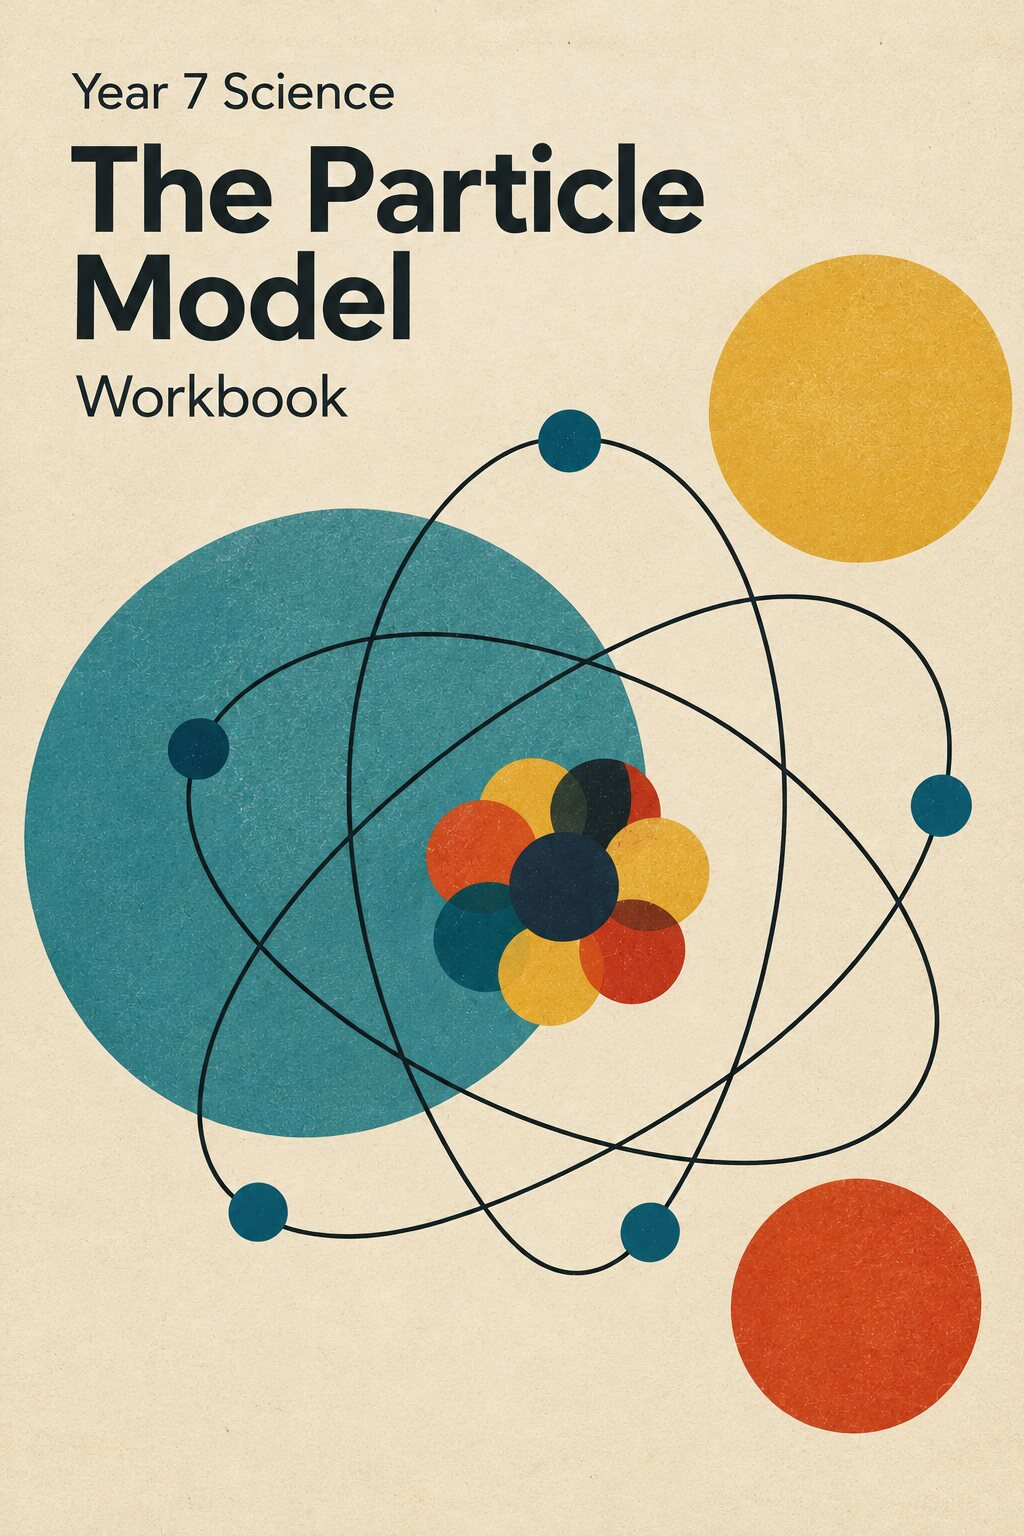
\includegraphics[width=\paperwidth]{../../../covers/particle-model.jpg}};
  \node[anchor=north east, fill=white, draw=Ink, line width=0.6pt, rounded corners=1.2mm,
        inner xsep=2mm, inner ysep=1.8mm, text width=30mm, font=\headingfont\footnotesize]
    at ([xshift=-4mm, yshift=-4mm]current page.north east)
    {\textbf{Name}\par\vspace{4mm}\hrule\vspace{2mm}\textbf{Class}\par\vspace{4mm}\hrule};
  \node[anchor=south east, fill=white, draw=Ink, line width=0.6pt, rounded corners=1.2mm,
        inner xsep=2.6mm, inner ysep=2mm, font=\headingfont\bfseries, align=right]
    at ([xshift=-4mm, yshift=6mm]current page.south east)
    {Advanced Particle Model 2\\[-1pt]{\normalfont\headingfont\scriptsize Topics 4--6}};
\end{tikzpicture}
\mbox{}
\clearpage

% ---- Inside cover ---------------------------------------------------------
\thispagestyle{plain}
{\headingfont\bfseries\fontsize{22}{26}\selectfont Advanced Particle Model}\par\vspace{1mm}
{\headingfont\large Book 2 \textbullet\ Topics 4--6 \textbullet\ Above the Year 7 level}\par\vspace{1mm}
{\small\itshape VC 2.0: VC2S8U05 \textbullet\ VC2S10U14 \textbullet\ VC2S10U15}\par\vspace{4mm}
\textbf{Teacher}\ \hrulefill\par

\begin{countrybox}{Acknowledgement of Country}
This booklet was created on the unceded Country of the Wurundjeri Woi-wurrung people of the Kulin Nation. We acknowledge Elders past, present and emerging.
\end{countrybox}

\begin{infobox}{How this booklet works}
\textbf{Advanced Particle Model} goes deeper into the ideas of the lesson books: more powerful models, the reasoning behind them, and harder problems that bring several ideas together. Each topic builds on the lessons named under its title. Each opens with its key vocabulary, then:\par\smallskip
\renewcommand{\arraystretch}{1.25}
\begin{tabular}{@{}p{24mm}p{70mm}@{}}
\textbf{Part A} & a reading with comprehension questions \\
\textbf{Part B} & the deeper idea, worked through \\
\textbf{Part C} & practice on your own \\
\textbf{Part D} & a challenge that pulls the ideas together \\
\end{tabular}

\smallskip
\begin{tabular}{@{}p{24mm}p{70mm}@{}}
\textbf{I do} \tagicon{\icodots{1}} & a worked example (solid frame) \\
\textbf{We do} \tagicon{\icodots{2}} & you try one with help (dashed frame) \\
\textbf{Reading} \tagicon{\icoread} & a passage to read (thin frame) \\
\end{tabular}
\end{infobox}

\clearpage
\markboth{Contents}{Contents}
{\headingfont\bfseries\LARGE Contents}\par\vspace{1mm}\noindent\rule{\linewidth}{0.6pt}\par\vspace{2mm}
\renewcommand{\arraystretch}{1.45}
\begin{tabular}{|C{1.1cm}|L{5.2cm}|C{1.7cm}|C{1.4cm}|}
  \hline\thead{Topic} & \thead{Title} & \thead{Deepens lesson} & \thead{Page} \\ \hline
  1 & \textit{Strange States of Matter} & 1 & Book 1 \\ \hline
  2 & \textit{Models and Their Limits} & 2, 4 & Book 1 \\ \hline
  3 & \textit{Particles, Energy and Temperature} & 4 & Book 1 \\ \hline
  4 & \hyperlink{lesson.4.1}{Energy and Changes of State} & 5 & \hyperlink{lesson.4.1}{p.\ \pageref{sec:4}} \\ \hline
  5 & \hyperlink{lesson.5.1}{Gas Pressure} & 7 & \hyperlink{lesson.5.1}{p.\ \pageref{sec:5}} \\ \hline
  6 & \hyperlink{lesson.6.1}{Density, Floating and Buoyancy} & 8 & \hyperlink{lesson.6.1}{p.\ \pageref{sec:6}} \\ \hline
  --- & \hyperlink{glossary}{Glossary} & & \hyperlink{glossary}{\pageref{sec:glossary}} \\ \hline
\end{tabular}
\renewcommand{\arraystretch}{1}
\clearpage
\setcounter{section}{3}\renewcommand{\lessonart}{7}
\sectiondiv{Energy and Changes of State}{Why the temperature stops rising \textbullet{} Heating and cooling curves \textbullet{} Latent heat by numbers \textbullet{} Pressure and boiling}\label{sec:4}
\lessoncodes{Deepens Lesson 5 \textbullet{} VC2S8U05 \textbullet{} VC2S10U15}

\vocabhead
\begin{ctab}
\begin{tabular}{|SW{3.4cm}|W{7.0cm}|}
  \hline\hd & \thead{Word} & \thead{Definition (copy from the slide)} \\ \hline
  & \scaf{\textbf{Heating curve}\label{voc:heating-curve}} & \scaf{A graph of temperature against time as a substance is heated.} \\ \hline
  & \textbf{Latent heat}\label{voc:latent-heat} & \\ \hline
  & \textbf{Plateau}\label{voc:plateau} & \\ \hline
  & \textbf{Sublimation}\label{voc:sublimation} & \\ \hline
  & \textbf{Pressure cooker}\label{voc:pressure-cooker} & \\ \hline
\end{tabular}
\end{ctab}

\lessonpart{A}{Reading and comprehension}{Teal}\label{read:4}

\begin{readingbox}{Reading --- Where Does the Energy Go?}
Put a pot of ice on a stove and measure its temperature every minute. The temperature climbs to 0\,\textdegree C and then stops, even though the stove is still heating it. It stays at 0\,\textdegree C until all the ice has melted. Then it climbs again, to 100\,\textdegree C, and stops again while the water boils. A graph of these readings is a \textbf{heating curve}, and the flat parts are \textbf{plateaus}.

Where does the energy go during a plateau? It is not making the particles move faster, so the temperature does not rise. Instead it is used to pull the particles apart against the attractions holding them together: from a fixed pattern into a liquid, or from a liquid into a gas. Energy used in this way is called \textbf{latent heat}, from a Latin word for ``hidden''.

Boiling point depends on the air pressure. High on a mountain, the air presses less on the water, so particles escape more easily and water boils below 100\,\textdegree C. A \textbf{pressure cooker} does the reverse: it traps steam, raises the pressure, and lets water reach about 120\,\textdegree C, so food cooks faster. Some solids skip the liquid state entirely: dry ice turns straight from solid to gas. This is \textbf{sublimation}.
\end{readingbox}

\rcreset
\rcq{Describe what happens to the temperature of ice as it is heated to boiling.}{2.5cm}
\rcq{During a plateau, what is the energy from the stove doing?}{2.5cm}
\rcq{Why does water boil below 100\,\textdegree C on a high mountain?}{2.5cm}
\rcq{How does a pressure cooker cook food faster?}{2.5cm}

\lessonpart{B}{Theory and examples}{Blue}\label{theory:4}

\subsection{Reading a Heating Curve}\label{sub:a4.1}

\begin{center}
\begin{fitbox}\begin{tikzpicture}[font=\small, x=0.55cm, y=0.032cm]
  \draw[->, line width=0.7pt] (0,-30) -- (16,-30) node[below left, font=\scriptsize] {time (min)};
  \draw[->, line width=0.7pt] (0,-30) -- (0,130) node[above right, font=\scriptsize] {temperature (\textdegree C)};
  \foreach \y in {-20,0,50,100} \draw (-0.15,\y) -- (0,\y) node[left, font=\scriptsize] {\y};
  \draw[line width=1.2pt] (0,-20) -- (1.5,0) -- (5,0) -- (8,100) -- (13.5,100) -- (15,125);
  \node[font=\scriptsize] at (1.0,15) {P};
  \node[font=\scriptsize] at (3.3,10) {Q};
  \node[font=\scriptsize] at (6.0,55) {R};
  \node[font=\scriptsize] at (10.8,110) {S};
  \node[font=\scriptsize] at (14.0,125) {T};
\end{tikzpicture}\end{fitbox}
\figcap{Heating ice from $-20$\,\textdegree C until it has all boiled.}
\end{center}

\begin{workedex}{What is happening in each section?}
\textbf{P:} ice warming; particles vibrate faster. \quad \textbf{Q:} plateau at 0\,\textdegree C; ice melting, energy pulling particles out of their fixed pattern. \quad \textbf{R:} liquid water warming; particles move faster. \quad \textbf{S:} plateau at 100\,\textdegree C; water boiling, energy separating particles completely. \quad \textbf{T:} steam warming.
\end{workedex}

\begin{wedo}{A cooling curve}
Hot liquid wax cools from 90\,\textdegree C. Its temperature falls steadily, stays at 54\,\textdegree C for six minutes, then falls again to room temperature. Sketch the cooling curve, label the freezing point, and state what the particles are doing during the flat part. Is energy being taken in or given out there?
\drawbox{6cm}{}
\end{wedo}

\subsection{Latent Heat by Numbers}\label{sub:a4.2}

\begin{skillbox}{Energy to change state}
\[ \text{energy (J)} = \text{mass (g)} \times \text{latent heat (J/g)} \]
For water: melting needs 334\,J for every gram; boiling needs 2260\,J for every gram.
\end{skillbox}

\begin{workedex}{Melting and boiling 50\,g}
Melt 50\,g of ice: $50 \times 334 = 16\,700$\,J.\\
Boil away 50\,g of water: $50 \times 2260 = 113\,000$\,J, almost seven times as much.

\smallskip
Melting only loosens the particles; they still touch. Boiling must pull every particle completely away from its neighbours, which takes far more energy.
\end{workedex}

\begin{wedo}{An ice tray}
An ice tray holds 200\,g of water. How much energy must the freezer remove to freeze it once it is at 0\,\textdegree C? How much energy would boil the same water away?
\workbox{5cm}
\end{wedo}

\lessonpart{C}{Practice}{Amber}\label{prac:4}

\begin{keepext}
\needspace{10\baselineskip}
\task Salt is spread on icy roads in cold countries. Salty water can stay liquid down to about $-10$\,\textdegree C, instead of freezing at 0\,\textdegree C. Explain why this makes the roads safer on a $-5$\,\textdegree C morning.
\answerbox{2.8cm}
\end{keepext}

\begin{keepext}
\needspace{10\baselineskip}
\task A pure substance has a sharp melting point. A mixture, like chocolate or candle wax, melts gradually over a range of temperatures. Suggest how you could use a melting point test to check whether a sample of a white powder is pure.
\answerbox{3.0cm}
\end{keepext}

\begin{keepext}
\needspace{10\baselineskip}
\task A drink is cooled with 100\,g of ice instead of 100\,g of cold water, both at 0\,\textdegree C. Which cools the drink more? Explain using the energy needed to melt ice.
\answerbox{3.0cm}
\end{keepext}

\begin{keepext}
\needspace{10\baselineskip}
\task Gallium is a metal that melts at about 30\,\textdegree C. A gallium spoon is used to stir a cup of hot tea at 70\,\textdegree C. Predict what happens, and explain using particles.
\answerbox{3.0cm}
\end{keepext}
\begin{keepext}
\needspace{10\baselineskip}
\task Sweating cools you down. Use the idea that the \emph{fastest} particles escape when water evaporates to explain why the sweat left behind on your skin gets cooler.
\answerbox{3.0cm}
\end{keepext}

\begin{keepext}
\needspace{10\baselineskip}
\task At the top of Mount Everest, water boils at about 70\,\textdegree C because the air pressure is much lower.
\pt{a}How many degrees lower is this than at sea level?
\workbox{1.6cm}
\pt{b}Climbers say it is very hard to cook pasta there. Explain why.
\answerbox{2.2cm}
\end{keepext}

\begin{keepext}
\needspace{10\baselineskip}
\task Ethanol boils at 78\,\textdegree C and water at 100\,\textdegree C. A spill of ethanol dries off a bench much faster than a spill of water. Suggest a particle reason for both facts.
\answerbox{3.0cm}
\end{keepext}

\begin{keepext}
\needspace{10\baselineskip}
\task Mothballs slowly get smaller in a wardrobe without ever becoming a puddle. Name the change of state and explain, using particles, what is happening.
\answerbox{2.8cm}
\end{keepext}


\lessonpart{D}{Challenge}{Violet}\label{ext:4}

\task A burn from steam at 100\,\textdegree C is much worse than a splash of boiling water at 100\,\textdegree C, even though they are at the same temperature. Explain why, using latent heat. Then calculate how much more energy 1\,g of steam gives your skin than 1\,g of boiling water, when each ends up as water at 100\,\textdegree C.
\answerbox{8cm}

\clearpage

% ══════════════════════════════════════════════════════════════════════════════
%  TOPIC 5 — GAS PRESSURE                                    (deepens Lesson 7)
%  The master's Lesson 12, whole.
% ══════════════════════════════════════════════════════════════════════════════
\setcounter{section}{4}\renewcommand{\lessonart}{12}
\sectiondiv{Gas Pressure}{Pressure from particle collisions \textbullet{} Squashing a gas \textbullet{} Heating a sealed gas \textbullet{} Air pressure all around us}\label{sec:5}
\lessoncodes{Deepens Lesson 7 \textbullet{} VC2S8U05 \textbullet{} VC2S8I01}

\vocabhead
\begin{ctab}
\begin{tabular}{|SW{2.91cm}|W{8.05cm}|}
  \hd & \thead{Word} & \thead{Definition (copy from the slide)} \\ \hline
  & \scaf{\textbf{Gas pressure}\label{voc:gas-pressure}} & \scaf{The push of a gas on the walls of its container, caused by particles hitting them.} \\ \hline
  & \textbf{Collision}\label{voc:collision} & \\ \hline
  & \textbf{Air pressure}\label{voc:air-pressure} & \\ \hline
  & \textbf{Sealed}\label{voc:sealed} & \\ \hline
  & \textbf{Kilopascal (kPa)}\label{voc:kilopascal-kpa} & \\ \hline
  & \textbf{Vacuum}\label{voc:vacuum} & \\ \hline
\end{tabular}
\end{ctab}

% ─── PART A ───────────────────────────────────────────────────────────────────
\lessonpart{A}{Reading and comprehension}{Teal}\label{read:12}

\begin{readingbox}{Reading --- Billions of Tiny Pushes}
Blow up a balloon and tie it off. What keeps it round? Inside, the air particles are moving in all directions at hundreds of metres per second. Every second, a huge number of them crash into the rubber. Each \textbf{collision} is a tiny push. Together, all those pushes make a steady force on every part of the balloon. This is \textbf{gas pressure}.

Gas pressure is measured in \textbf{kilopascals}, written kPa. A car tyre might be pumped to about 220\,kPa more than the air outside. To raise the pressure in a \textbf{sealed} container --- one that nothing can get into or out of --- you need more collisions with the walls each second, or harder ones. Squashing the gas into a smaller space does the first: the particles have less room, so they hit the walls more often. Heating the gas does both: the particles move faster, so they hit the walls more often and harder.

You live at the bottom of a deep ocean of air. The weight of all that air above you causes \textbf{air pressure}, about 101\,kPa at sea level. You do not feel it because the air inside your body pushes out just as hard. But take the air out of one side of something and you can see its power. In a \textbf{vacuum} there are no particles at all, so there is no pressure. A drink can with the air sucked out of it is crushed flat by the air pressure outside.
\end{readingbox}

\rcreset
\rcq{What keeps a blown-up balloon round?}{1.8cm}
\rcq{What is a collision, and how does it make pressure?}{1.8cm}
\rcq{What unit is gas pressure measured in?}{1.2cm}
\rcq{Give two ways to make more collisions with the walls of a sealed container.}{1.8cm}
\rcq{Why does heating a gas make its particles hit the walls harder?}{1.6cm}
\rcq{What causes air pressure?}{1.6cm}
\rcq{Why don't you feel the air pressure pushing on you?}{1.6cm}
\rcq{Why is there no pressure in a vacuum?}{1.4cm}

% ─── PART B ───────────────────────────────────────────────────────────────────
\lessonpart{B}{Theory and examples}{Blue}\label{theory:12}

\subsection{Pressure From Particle Collisions}\label{sub:12.1}

\begin{center}\begin{fitbox}\begin{fitbox}\begin{tikzpicture}[font=\small]
  \begin{scope}
    \foreach \x/\y in \gaspos{\node[pA] at (\x,\y) {};}
    \gasMoves \pbox
    \foreach \y in {0.6,1.4,2.1}{\draw[OrangeDark, line width=1pt, -{Stealth[length=4pt]}] (2.6,\y) -- (3.0,\y);}
    \foreach \x in {0.7,1.9}{\draw[OrangeDark, line width=1pt, -{Stealth[length=4pt]}] (\x,2.6) -- (\x,3.0);}
    \node[lab, font=\small, anchor=west] at (3.2,1.4) {each collision pushes on the wall};
  \end{scope}
\end{tikzpicture}\end{fitbox}\end{fitbox}\end{center}
\figcap{Particles hitting the walls of a sealed container push outwards in every direction.}

\begin{infobox}{More pressure means\ldots}
\textbf{more} collisions with the walls each second, \textbf{or} \textbf{harder} collisions, \textbf{or} both.
\end{infobox}

\subsection{Squashing a Gas}\label{sub:12.2}

\begin{center}\begin{fitbox}\begin{fitbox}\begin{tikzpicture}[font=\small]
  \begin{scope}
    \foreach \x/\y in \gaspos{\node[pA] at (\x,\y) {};}\pbox
    \node[font=\small\bfseries, text=NavyBlue] at (1.3,-0.35) {before};
  \end{scope}
  \draw[thin arrow, DarkGrey] (3.0,1.3) -- node[above, font=\scriptsize] {squash} (3.9,1.3);
  \begin{scope}[xshift=4.3cm]
    \foreach \x/\y in {0.35/0.3,0.95/0.35,1.55/0.3,2.2/0.4,0.6/0.85,1.25/0.9,1.9/0.95,2.3/1.1}{\node[pA] at (\x,\y) {};}
    \draw[boxline] (0,0) rectangle (2.6,1.3);
    \draw[line width=3pt, DarkGrey] (-0.1,1.38) -- (2.7,1.38);
    \node[font=\small\bfseries, text=NavyBlue] at (1.3,-0.35) {after: same particles, half the space};
  \end{scope}
\end{tikzpicture}\end{fitbox}\end{fitbox}\end{center}

\begin{workedex}{Squashing a gas}
You put your finger over the end of a bicycle pump and push the handle in. It gets harder and harder to push. Explain, using particles.

\medskip
The same number of air particles are squeezed into a \textbf{smaller space}. They hit the walls and the plunger \textbf{more often}, so the \textbf{pressure rises}. The higher pressure pushes back harder on the handle.
\end{workedex}

\begin{wedo}{Squashing a gas}
A diver breathes out a bubble of air deep underwater. As the bubble rises towards the surface, the water pressure on it gets smaller and the bubble gets bigger. Explain, using particles, why the bubble is smaller when it is deeper.
\answerbox{3.2cm}
\end{wedo}

\subsection{Heating a Sealed Gas}\label{sub:12.3}

\begin{workedex}{Heating a sealed gas}
An aerosol can carries the warning ``Do not heat or throw into a fire.'' Explain why, using particles.

\medskip
Heating gives the gas particles inside more \textbf{kinetic energy}, so they move faster. They hit the inside of the can \textbf{more often} and \textbf{harder}, so the pressure rises. The can is sealed, so the pressure keeps building until the can could burst.
\end{workedex}

\begin{wedo}{Cooling a sealed gas}
A car's tyre pressure is lower on a cold morning than in the afternoon, even though no air has leaked out. Explain, using particles.
\answerbox{3.2cm}
\end{wedo}

% ─── PART C ───────────────────────────────────────────────────────────────────
\lessonpart{C}{Practice}{Amber}\label{prac:12}

Work through every task. In each explanation, say what happens to the number or the force of the collisions.

\needspace{12\baselineskip}
\task Write whether the pressure goes \textbf{UP} or \textbf{DOWN}.

\vspace{4pt}
\begin{ctab}
\begin{tabular}{|SW{3.99cm}|Z{1.20cm}|W{3.73cm}|Z{1.20cm}|}
  \hd & \thead{Change} & \thead{Up or down?} & \thead{Change} & \thead{Up or down?} \\ \hline
  & A sealed syringe is pushed in & \scaf{UP} & A balloon is put in the fridge & \scaf{DOWN} \\ \hline
  & A sealed jar is left in the sun & & A sealed syringe is pulled out & \\ \hline
  & More air is pumped into a tyre & & Air is let out of a tyre & \\ \hline
\end{tabular}
\end{ctab}

\taskpair{Explain what causes the pressure of the air inside a football.}{2.8cm}
         {Explain why it is harder to push in a sealed syringe the further you push.}{2.8cm}

\needspace{10\baselineskip}
\task Explain, using particles, why a balloon left in a hot car might burst.
\answerbox{3.0cm}

\needspace{10\baselineskip}
\task A packet of chips is sealed at the beach. It is driven up a high mountain, where the air pressure outside is lower, and the packet puffs up. Explain why.
\answerbox{3.0cm}

\needspace{10\baselineskip}
\task Tom says, ``When you heat a gas in a sealed can, the particles get bigger and push on the walls.'' Explain what is wrong with Tom's idea, and give the correct explanation.
\answerbox{3.0cm}

\needspace{10\baselineskip}
\task A teacher heats a little water in an open can until steam comes out, then quickly turns the can upside down into a bowl of cold water. The can is crushed with a bang.
\pt{a}What happens to the steam inside the can when it touches the cold water?
\answerbox{1.8cm}
\pt{b}Explain why the can is crushed.
\answerbox{2.4cm}

% ─── PART D ───────────────────────────────────────────────────────────────────
\needspace{14\baselineskip}\par\medskip{\headingfont\bfseries\large More practice}\par\smallskip
\begin{keepext}
\needspace{10\baselineskip}
\task Oxygen moves from the air in your lungs into your blood by diffusion. The air in the lungs has a high concentration of oxygen; blood arriving at the lungs has a low concentration. Explain why breathing in fresh air keeps the oxygen moving into the blood.
\answerbox{3.2cm}
\end{keepext}

\begin{keepext}
\needspace{10\baselineskip}
\task Design a fair test to find out whether diffusion is faster in water or in cooking oil. Name what you would change, what you would measure and two things you would keep the same.
\answerbox{3.4cm}
\end{keepext}

\begin{keepext}
\needspace{10\baselineskip}
\task Perfume particles are much heavier than the particles of a strong-smelling gas called ammonia. Predict which would spread across a room faster, and give a particle reason.
\answerbox{2.8cm}
\end{keepext}

\begin{keepext}
\needspace{10\baselineskip}
\task A gold block and a lead block were clamped tightly together for several years. When they were separated, a tiny amount of gold had moved into the lead. What does this suggest about diffusion in solids?
\answerbox{2.8cm}
\end{keepext}
\begin{keepext}
\needspace{10\baselineskip}
\task A steel rail gets 0.012\,mm longer for every metre of length, for every 1\,\textdegree C it warms up. A 20\,m rail warms from 10\,\textdegree C to 40\,\textdegree C. How much longer does it get? Show your working.
\workbox{3.0cm}
\end{keepext}

\begin{keepext}
\needspace{10\baselineskip}
\task A bimetallic strip is made of brass and steel joined together. Brass expands more than steel. Predict which way the strip bends when it is heated, and explain why. Sketch it if it helps.
\answerbox{3.2cm}
\end{keepext}

\begin{keepext}
\needspace{10\baselineskip}
\task Thick glass cups sometimes crack when boiling water is poured into them, but thin laboratory glass does not. Suggest why, using the idea that the inside of the glass heats up before the outside.
\answerbox{3.0cm}
\end{keepext}

\begin{keepext}
\needspace{10\baselineskip}
\task Water is unusual. Between 0\,\textdegree C and 4\,\textdegree C it \emph{contracts} as it warms, instead of expanding. A lake in winter has water at 4\,\textdegree C at the bottom and ice on top. Suggest why this helps fish survive the winter.
\answerbox{3.0cm}
\end{keepext}

\lessonpart{D}{Challenge}{Violet}
\begin{keepext}
\needspace{10\baselineskip}
\task At a fixed temperature, halving the volume of a gas doubles its pressure. A sealed syringe of air at 100\,kPa is pushed in from 60\,mL to 30\,mL, and then to 15\,mL. Find the pressure at each volume. Show your working.
\workbox{3.0cm}
\end{keepext}

\begin{keepext}
\needspace{10\baselineskip}
\task You drink through a straw by sucking some air out of the straw. Explain, using air pressure, what actually pushes the drink up the straw.
\answerbox{3.0cm}
\end{keepext}

\begin{keepext}
\needspace{10\baselineskip}
\task Your ears sometimes ``pop'' when a plane takes off. Inside your ear, behind the eardrum, is a small space of air. Use the idea of air pressure on each side of the eardrum to explain what you feel.
\answerbox{3.0cm}
\end{keepext}

\begin{keepext}
\needspace{10\baselineskip}
\task Space is almost a vacuum. Explain why astronauts need pressurised spacesuits, using the idea of the pressure inside the body pushing out.
\answerbox{3.0cm}
\end{keepext}


\clearpage

% ══════════════════════════════════════════════════════════════════════════════
%  TOPIC 6 — DENSITY, FLOATING AND BUOYANCY                  (deepens Lesson 8)
% ══════════════════════════════════════════════════════════════════════════════
\setcounter{section}{5}\renewcommand{\lessonart}{13}
\sectiondiv{Density, Floating and Buoyancy}{Rearranging $D = m \div V$ \textbullet{} Average density \textbullet{} Archimedes' principle \textbullet{} Ships and submarines}\label{sec:6}
\lessoncodes{Deepens Lesson 8 \textbullet{} VC2S8U05 \textbullet{} VC2S10I04}

\vocabhead
\begin{ctab}
\begin{tabular}{|SW{3.4cm}|W{7.0cm}|}
  \hline\hd & \thead{Word} & \thead{Definition (copy from the slide)} \\ \hline
  & \scaf{\textbf{Buoyant force}\label{voc:buoyant-force}} & \scaf{The upward push of a liquid or gas on an object in it.} \\ \hline
  & \textbf{Displace}\label{voc:displace} & \\ \hline
  & \textbf{Average density}\label{voc:average-density} & \\ \hline
  & \textbf{Archimedes' principle}\label{voc:archimedes-principle} & \\ \hline
  & \textbf{Ballast}\label{voc:ballast} & \\ \hline
\end{tabular}
\end{ctab}

\lessonpart{A}{Reading and comprehension}{Teal}\label{read:6}

\begin{readingbox}{Reading --- Why a Steel Ship Floats}
Drop a steel bolt into water and it sinks. Yet a steel cargo ship weighing tens of thousands of tonnes floats. The secret is the shape. A ship's steel is spread into a thin hull around a huge space filled with air, so the \textbf{average density} of the whole ship, its total mass divided by its total volume, is less than the density of water.

When anything is placed in water, it pushes some water out of the way: it \textbf{displaces} it. The water pushes back up with a \textbf{buoyant force}. Over two thousand years ago, Archimedes worked out how big that force is. \textbf{Archimedes' principle} says the buoyant force equals the weight of the water displaced. A ship sinks into the water until it has displaced its own weight of water, then floats.

Sea water is denser than fresh water, so a ship floats a little higher at sea than in a river. A submarine controls whether it floats or sinks with \textbf{ballast} tanks: it lets sea water in to raise its average density and dive, and blows the water out with compressed air to rise.
\end{readingbox}

\rcreset
\rcq{Why does a steel ship float when a steel bolt sinks?}{2.5cm}
\rcq{State Archimedes' principle in your own words.}{2.5cm}
\rcq{Why does a ship float higher in sea water than in fresh water?}{2.5cm}
\rcq{How does a submarine change its average density to dive and rise?}{2.5cm}

\lessonpart{B}{Theory and examples}{Blue}\label{theory:6}

\subsection{Rearranging the Density Formula}\label{sub:a6.1}

\begin{skillbox}{Three forms of one rule}
\[ D = \frac{m}{V} \qquad m = D \times V \qquad V = \frac{m}{D} \]
Cover the quantity you want: what is left tells you whether to multiply or divide. Keep the units matched: g and cm\textsuperscript{3} give g/cm\textsuperscript{3}.
\end{skillbox}

\begin{workedex}{Finding a mass}
A copper block has a volume of 20\,cm\textsuperscript{3}. Copper has a density of 8.9\,g/cm\textsuperscript{3}. Find the mass.

\smallskip
$m = D \times V = 8.9 \times 20 = \mathbf{178\,g}$.
\end{workedex}

\begin{wedo}{Finding a volume}
A piece of cork has a mass of 12\,g. Cork has a density of 0.24\,g/cm\textsuperscript{3}. Find its volume.
\workbox{4cm}
\end{wedo}

\subsection{Will It Float?}\label{sub:a6.2}

\begin{workedex}{A sealed drum}
A sealed steel drum has a volume of 200\,000\,cm\textsuperscript{3} (200\,L) and a mass of 20\,kg (20\,000\,g). Does it float in fresh water (1\,g/cm\textsuperscript{3}), and how much cargo can it hold before it sinks?

\smallskip
Average density $= 20\,000 \div 200\,000 = \mathbf{0.1\ g/cm^3}$, less than water, so it floats.
It sinks when its average density reaches 1\,g/cm\textsuperscript{3}, that is, when its total mass reaches $1 \times 200\,000 = 200\,000$\,g. So it can carry $200\,000 - 20\,000 = 180\,000$\,g, or \textbf{180\,kg} of cargo.
\end{workedex}

\begin{wedo}{A canoe}
A canoe has a mass of 30\,kg and, if it were filled to the brim, would hold 300\,L (300\,000\,cm\textsuperscript{3}). What is the greatest total mass of paddlers and gear it could carry before water comes over the side? What happens to that answer in sea water (1.03\,g/cm\textsuperscript{3})?
\workbox{5.5cm}
\end{wedo}

\lessonpart{C}{Practice}{Amber}\label{prac:6}

\begin{keepext}
\needspace{10\baselineskip}
\task Steel has a density of 7.9\,g/cm\textsuperscript{3}, yet huge steel ships float. A ship is mostly air inside. Explain how a steel ship can float, using the idea of the density of the whole ship.
\answerbox{3.2cm}
\end{keepext}

\begin{keepext}
\needspace{10\baselineskip}
\task A hot-air balloon rises when the air inside it is heated. Explain, using particles and density, why hot air rises through cold air.
\answerbox{3.2cm}
\end{keepext}

\begin{keepext}
\needspace{10\baselineskip}
\task An egg sinks in tap water but floats in very salty water. What does this tell you about the density of the egg compared with each liquid? Explain.
\answerbox{3.0cm}
\end{keepext}

\begin{keepext}
\needspace{10\baselineskip}
\task Most substances are denser as solids than as liquids, but ice is less dense than water. Predict what would happen to a lake in winter if ice were denser than water, and why that would matter for living things.
\answerbox{3.0cm}
\end{keepext}
\begin{keepext}
\needspace{10\baselineskip}
\task A 50\,cm\textsuperscript{3} block of aluminium has a density of 2.7\,g/cm\textsuperscript{3}. Find its mass.
\workbox{2.6cm}
\end{keepext}

\begin{keepext}
\needspace{10\baselineskip}
\task A gold bar has a mass of 1000\,g. Gold has a density of 19.3\,g/cm\textsuperscript{3}. Find the volume of the bar, to one decimal place.
\workbox{2.6cm}
\end{keepext}

\begin{keepext}
\needspace{10\baselineskip}
\task King Hiero's crown had a mass of 1000\,g. A pure gold crown would have a volume of 51.8\,cm\textsuperscript{3}. Archimedes found its volume was 60\,cm\textsuperscript{3}.
\pt{a}Calculate the crown's density.
\workbox{2.2cm}
\pt{b}What does this tell you about the crown? Silver's density is 10.5\,g/cm\textsuperscript{3}.
\answerbox{2.2cm}
\end{keepext}

\begin{keepext}
\needspace{10\baselineskip}
\task Water has a density of 1\,g/mL. What is the mass of the water in a full 1.5\,L bottle? (1\,L = 1000\,mL.)
\workbox{2.4cm}
\end{keepext}


\needspace{10\baselineskip}
\task An egg sinks in a glass of tap water. As salt is stirred in, the egg slowly rises and then floats. Explain why, using density.
\answerbox{4.5cm}

\lessonpart{D}{Challenge}{Violet}\label{ext:6}

\task You need the density of a cork, which floats, so you cannot simply sink it in a measuring cylinder to find its volume. You also have a heavy metal sinker, string and a balance. Plan a method to find the cork's density, and show how you would calculate it from your measurements.
\answerbox{9cm}

\clearpage

\clearpage\markboth{Glossary}{Glossary}\hypertarget{glossary}{}\pdfbookmark[1]{Glossary}{glossarybm}
{\headingfont\bfseries\LARGE Glossary}\label{sec:glossary}\par\vspace{1mm}\noindent\rule{\linewidth}{0.6pt}\par
{\small Every key word in this booklet and the page it is introduced on.}\par\smallskip
\renewcommand{\arraystretch}{1.3}
\begin{longtable}{|>{\RaggedRight}p{34mm}|p{9mm}|p{\dimexpr\linewidth-43mm-6\tabcolsep-4\arrayrulewidth-1pt\relax}|}
\hline \rule{0pt}{4mm}\headingfont\bfseries Word & \headingfont\bfseries Page & \headingfont\bfseries In my own words \\ \hline \endhead
  Air pressure & \pageref{voc:air-pressure} & \\ \hline
  Archimedes' principle & \pageref{voc:archimedes-principle} & \\ \hline
  Average density & \pageref{voc:average-density} & \\ \hline
  Ballast & \pageref{voc:ballast} & \\ \hline
  Buoyant force & \pageref{voc:buoyant-force} & \\ \hline
  Collision & \pageref{voc:collision} & \\ \hline
  Displace & \pageref{voc:displace} & \\ \hline
  Gas pressure & \pageref{voc:gas-pressure} & \\ \hline
  Heating curve & \pageref{voc:heating-curve} & \\ \hline
  Kilopascal (kPa) & \pageref{voc:kilopascal-kpa} & \\ \hline
  Latent heat & \pageref{voc:latent-heat} & \\ \hline
  Plateau & \pageref{voc:plateau} & \\ \hline
  Pressure cooker & \pageref{voc:pressure-cooker} & \\ \hline
  Sealed & \pageref{voc:sealed} & \\ \hline
  Sublimation & \pageref{voc:sublimation} & \\ \hline
  Vacuum & \pageref{voc:vacuum} & \\ \hline
\end{longtable}
\padtofour
\end{document}
